\documentclass[pdflatex,sn-nature]{sn-jnl}% Style for submissions to Nature Portfolio journals

%%%% Standard Packages
\usepackage{graphicx}%
\usepackage{multirow}%
\usepackage{amsmath,amssymb,amsfonts}%
\usepackage[title]{appendix}%
\usepackage{xcolor}%
\usepackage{textcomp}%
\usepackage{manyfoot}%
\usepackage{booktabs}
\usepackage{longtable}        % multi-page supplementary tables
\usepackage{siunitx}          % decimal-aligned numeric columns
\sisetup{detect-all, table-align-text-before=false, table-align-text-after=false,
         input-symbols={()[]}, table-number-alignment=center}%
\usepackage{array}%
\usepackage{colortbl}%
\usepackage{amsthm}%
%%%%

\graphicspath{{figures/}}

%% Theorem environments (SN-provided numbered styles)
\theoremstyle{thmstyleone}
\newtheorem{theorem}{Theorem}
\newtheorem{lemma}{Lemma}
\newtheorem{proposition}{Proposition}
\newtheorem{corollary}{Corollary}
\theoremstyle{thmstylethree}
\newtheorem{definition}{Definition}
\theoremstyle{thmstyleone}

%% ---------------------------------------------------------------------------
%% Red flags for author-supplied items. Every unresolved item in this manuscript
%% is wrapped in one of these three and prints in red.
%% TO PRODUCE THE FINAL SUBMISSION PDF: set \finaltrue below. Every flag then
%% vanishes and any that is still unresolved will be obvious as a hole in the text.
%% ---------------------------------------------------------------------------
\newif\iffinal
\finalfalse                     % <-- set to \finaltrue for the submission PDF
\iffinal
  \newcommand{\MISSING}[1]{}
  \newcommand{\VERIFY}[1]{}
  \newcommand{\BLOCKING}[1]{}
  \long\def\REV#1{#1}
\else
  \newcommand{\MISSING}[1]{\textcolor{red}{[MISSING: #1]}}
  \newcommand{\VERIFY}[1]{\textcolor{red}{[VERIFY: #1]}}
  \newcommand{\BLOCKING}[1]{\textcolor{red}{[BLOCKING: #1]}}
  %% \REV marks text added or changed in this revision round. Setting \finaltrue
  %% above renders it as ordinary black text -- no unwrapping needed at submission.
  %% Declared \long so a marked span may cross paragraph breaks (\textcolor is not).
  \newcommand{\REVcolor}[1]{\textcolor{red}{#1}}
  \long\def\REV#1{\begingroup\color{red}#1\endgroup}
\fi

%% Line numbers for peer review (Nature Portfolio asks for numbered lines in the
%% review PDF). Comment out the \linenumbers line for the production version.
\usepackage[mathlines]{lineno}
\linenumbers
\makeatletter
\AtBeginDocument{\@ifpackageloaded{lineno}{%
  \setlength{\linenumbersep}{8pt}%
  \renewcommand\linenumberfont{\normalfont\scriptsize\color{gray}}%
  \leftlinenumbers}{}}
\makeatother

%% Cross-document references. xr imports the label table of the main manuscript,
%% so references from this SI to main-text items (e.g. Theorem \ref{thm:zero})
%% resolve to the numbers printed there. Build with ./build.sh: it extracts
%% main's \newlabel lines into main-labels.aux before every pass, so xr imports
%% labels only (importing the raw .aux would also import \bibcite lines and
%% clash with this document's own citation numbering). No prefix is needed
%% because the SI label namespaces do not collide with the main-text ones.
\usepackage{xr}
\externaldocument{main-labels}

%% Supplementary numbering: caption words "Supplementary Fig./Table",
%% plain-arabic numbers to match the main text's "Supplementary Fig.~N" references.
\renewcommand{\figurename}{Supplementary Fig.}
\renewcommand{\tablename}{Supplementary Table}

%% Convenience macros for naming SI items, mirroring main.tex so the shared
%% section file sections/supplementary.tex compiles identically in both documents.
\newcommand{\snote}[1]{Supplementary Note~\ref{#1}}
\newcommand{\stab}[1]{Supplementary Table~\ref{#1}}
\newcommand{\sfig}[1]{Supplementary Fig.~\ref{#1}}
\newcommand{\stabs}[2]{Supplementary Tables~\ref{#1}--\ref{#2}}

%% Auto-numbered Supplementary Notes so cross-references resolve via \ref.
%% \suppnote{Title} prints "Supplementary Note N: Title" and is \label-able
%% (the following \label picks up the note number through \refstepcounter).
\newcounter{suppnote}
\newcommand{\suppnote}[1]{%
  \refstepcounter{suppnote}%
  \section*{Supplementary Note \thesuppnote: #1}%
}

\raggedbottom

\begin{document}

\title[Supplementary Information]{Supplementary Information for\\ Parity-blind equivariant networks predict physically impossible material properties}

\author[1]{\fnm{Can} \sur{Polat}}% ORCID: 0000-0002-1458-302X

\author*[2,3]{\fnm{Mustafa} \sur{Kurban}}\email{kurbanm@ankara.edu.tr}% ORCID: 0000-0002-7263-0234

\author[1]{\fnm{Erchin} \sur{Serpedin}}% ORCID: 0000-0001-9069-770X

\author*[4]{\fnm{Hasan} \sur{Kurban}}\email{hkurban@hbku.edu.qa}% ORCID: 0000-0003-3142-2866

\affil[1]{\orgdiv{Department of Electrical and Computer Engineering}, \orgname{Texas A\&M University}, \orgaddress{\city{College Station}, \state{Texas}, \country{USA}}}

\affil[2]{\orgdiv{Department of Electrical and Computer Engineering}, \orgname{Texas A\&M University at Qatar}, \orgaddress{\city{Doha}, \country{Qatar}}}

\affil[3]{\orgdiv{Department of Prosthetics and Orthotics}, \orgname{Ankara University}, \orgaddress{\city{Ankara}, \country{Turkey}}}

\affil[4]{\orgdiv{College of Science and Engineering}, \orgname{Hamad Bin Khalifa University}, \orgaddress{\city{Doha}, \country{Qatar}}}

\maketitle

% Supplementary Information body. Compiled standalone via sn-supplementary.tex.
% Eight Supplementary Notes, ordered by first citation in the main text. Labels for
% the folded notes (snote:rawvariant, snote:stats, snote:inversion, snote:frozen,
% snote:eqv2, snote:excluded) sit inside the note that now contains them and resolve
% to that note's number, so no main-text citation needs rewriting.
\setlength{\tabcolsep}{3pt}

% ===== Note 1 =====
\suppnote{Proofs, construction of the SO(3) arms, and the verification gate}\label{snote:proofs}

Every statement proved here is stated in full, with its assumptions, in the main text. This note supplies the numerical evidence for the assumptions, the proofs, and the crystallographic classification that turns Corollary~1 into a quantitative ceiling.

\subsection*{The assumptions, and the evidence for them}

The main text assumes (A1) permutation invariance, (A2) translation invariance under a rigid shift by any vector as well as under lattice translations, and (A3) $G$-equivariance. The first two hold by construction for every architecture in this study: each reads out a sum of per-atom or per-edge contributions on a graph built from lattice-periodic displacement vectors, and a sum is invariant to the order of its terms. They are also measured. On centrosymmetric inputs the relative residual $\lVert f(I\!\cdot\!x)-f(x)\rVert/\lVert f(x)\rVert$ is at most $10^{-6}$ for the three matched cores (Supplementary Note~\ref{snote:inversion}). (A3) is measured at both the feature level, before training (Supplementary Table~\ref{stab:gate}), and the output level, after training (Supplementary Note~\ref{snote:eqv2}). EqV2 is the exception and is treated as such: it satisfies (A1)--(A2) only to $0.10$--$0.15$ and (A3) only to $7$--$11\%$, so the exact statements below apply to it only through their stability clauses, which is measurable and is measured, as follows.

All four defects were measured directly on the evaluation population for every arm and seed. For Proposition~1, over the 2,000 idealized structures the median absolute defects are $\delta \le 8\times10^{-7}$ and $\eta \le 8\times10^{-7}$ for the NequIP and Allegro O(3) arms ($\delta \le 6\times10^{-6}$, $\eta \le 5\times10^{-7}$ for MACE, whose weights are single precision), and the observed violation lies below the measured floor $(\delta+\eta)/2$ on every structure of every run; the floor is not loose, with median violations at $60$--$70\%$ of the median bound, so the O(3) residuals are fully accounted for by arithmetic. For the SO(3) arms $\delta$ stays below $5\times10^{-6}$ while $\eta$ has medians $1.2$--$2.2$, so the same inequality bounds nothing there, which is exactly the freedom the headline measures. For EqV2, $\delta$ (median $0.055$) and $\eta$ ($0.73$--$1.08$) give a floor of $0.40$--$0.57$ against observed medians of $0.36$--$0.54$: its violations are quantitatively its measured defects. For the stability clause of Corollary~1, $\delta_{+}$ and $\epsilon$ were measured over the full proper subgroup of every m$\bar 3$m crystal (23 rotations each, spglib operations converted to Cartesian). The matched SO(3) cores have $\delta_{+}$ medians of $3.6\times10^{-7}$ to $2.2\times10^{-6}$ with m$\bar 3$m violation medians of the same order, and the bound $\delta_{+}/(1-\epsilon)$ holds on every structure where it applies; on most m$\bar 3$m structures $\epsilon \ge 1$ numerically, because the relative error divides a machine-zero prediction, and there the equivalent absolute form $\lVert f(x)\rVert_F \le \delta_{+} + \max_{R}\lVert f(R\!\cdot\!x) - D(R)f(x)\rVert_F$, from the same averaging argument without the rearrangement, holds on all 166 crystals for every arm and seed. For EqV2 the clause is quantitative rather than vacuous: its m$\bar 3$m violation medians, $0.9$--$1.4\times10^{-2}$, lie below its measured $\delta_{+}$ medians of $1.8$--$3.0\times10^{-2}$. The m$\bar 3$m signal it reports is therefore its own (A1)--(A2) defect, as the clause predicts.

\subsection*{Definition 1 and Lemma 1}

\begin{definition}[Centrosymmetric structure]\label{sdef:centro}
With the inversion centre at the origin, a species-preserving involution $\pi$ of the atoms and lattice vectors $\mathbf{t}_i \in \Lambda$ satisfy $-\mathbf{r}_i = \mathbf{r}_{\pi(i)} + \mathbf{t}_i$ for every $i$.
\end{definition}

\begin{lemma}[Inversion identity]\label{slem:inv}
Let $f_\theta$ satisfy (A1) and (A2). Then $f_\theta(I\!\cdot\!x) = f_\theta(x)$ for every centrosymmetric $x$ and every $\theta$.
\end{lemma}

\begin{proof}
Place the inversion centre at the origin; by (A2) this is a choice of coordinates and not an assumption, so inverting about the cell origin instead, as the experiments do, changes the result by a rigid shift and hence not at all. By Definition~\ref{sdef:centro}, the inverted structure $I\!\cdot\!x$ has its atoms at $-\mathbf{r}_i = \mathbf{r}_{\pi(i)} + \mathbf{t}_i$. Discarding the lattice translations $\mathbf{t}_i$ by (A2) and relabelling atom $i$ as $\pi(i)$ by (A1), which is species-preserving, $I\!\cdot\!x$ and $x$ are the same input to $f_\theta$. Hence $f_\theta(I\!\cdot\!x) = f_\theta(x)$. No property of $\theta$, and no assumption about parity, is used.
\end{proof}

\subsection*{Theorem 1: the structural zero}

\begin{theorem}[Structural zero]\label{sthm:zero}
Let $f_\theta$ satisfy (A1), (A2) and (A3) with $G=\mathrm{O}(3)$, and let the target be a rank-$r$ polar tensor with $r$ odd. Then $f_\theta(x)=0$ for every centrosymmetric $x$ and every $\theta$.
\end{theorem}

\begin{proof}
Lemma~\ref{slem:inv} gives $f_\theta(I\!\cdot\!x) = f_\theta(x)$. Assumption (A3) at $Q = I$ gives
$f_\theta(I\!\cdot\!x) = D(I) f_\theta(x) = (-1)^{r} f_\theta(x) = -f_\theta(x)$, because $r$ is odd.
Equating the two, $f_\theta(x) = -f_\theta(x)$, so $2 f_\theta(x) = 0$ and $f_\theta(x) = 0$. The argument does not refer to $\theta$, to the training data, or to the loss.
\end{proof}

For $G=\mathrm{SO}(3)$ the second step is unavailable: (A3) is asserted for proper rotations only and $D(I)$ is never invoked. Nothing else in the construction changes; that is the entire content of the parity relabelling. The theorem also applies to the molecular dipole, $r=1$. It is nearly vacuous on QM9: symmetry forces the dipole to vanish for 7 of the 10,831 molecules in the evaluation population, or $0.065\%$ (\snote{snote:qm9pg}), which is why the dipole separates a parity-odd target from an active parity constraint (main-text Fig.~3).

\subsection*{Proposition 1: the arithmetic floor}

\begin{proposition}[Arithmetic floor]\label{sprop:floor}
Fix a centrosymmetric $x$, and let $\delta = \lVert f_\theta(I\!\cdot\!x) - f_\theta(x)\rVert_F$ and $\eta = \lVert f_\theta(I\!\cdot\!x) - D(I) f_\theta(x)\rVert_F$ measure the failure of (A1)--(A2) and of the O(3) law at $Q=I$. Then $\lVert f_\theta(x)\rVert_F \le \tfrac{1}{2}(\delta + \eta)$.
\end{proposition}

\begin{proof}
Since $D(I) = -\mathrm{id}$ for odd $r$,
\[
2 f_\theta(x) = \bigl[f_\theta(x) - f_\theta(I\!\cdot\!x)\bigr] + \bigl[f_\theta(x) + f_\theta(I\!\cdot\!x)\bigr],
\]
and the two brackets have norms $\delta$ and $\eta$ respectively. The triangle inequality gives $2\lVert f_\theta(x)\rVert_F \le \delta + \eta$.
\end{proof}

With $\delta=\eta=0$ the proposition recovers Theorem~\ref{sthm:zero}. In floating point $\delta$ and $\eta$ are set by the arithmetic, so an O(3) model's residual floor is bounded by half their sum and therefore tracks its precision, not its symmetry: this is why the measured O(3) floors sit at the single-precision level ($3\times10^{-7}$ to $3\times10^{-6}$\,C\,m$^{-2}$, Supplementary Table~\ref{stab:distribution}) and why MACE's is roughly eight times the others', its symmetric contractions remaining in single precision even under a double-precision cast (Supplementary Note~\ref{snote:construction}). Finally, for a parity-blind model Lemma~\ref{slem:inv} forces $f_\theta(I\!\cdot\!x)=f_\theta(x)$, hence $\delta=0$ and $\eta = 2\lVert f_\theta(x)\rVert_F$, and the bound reads $\lVert f_\theta(x)\rVert_F \le \lVert f_\theta(x)\rVert_F$. It is vacuous. The guarantee and its stability are lost together, which is the sharpest way to state what the missing label costs.

\subsection*{Corollary 1: the rotation ceiling}

\begin{corollary}[Rotation ceiling]\label{scor:rot}
Let $f_\theta$ satisfy (A1), (A2) and (A3) with $G = \mathrm{SO}(3)$, and let $G^{+}(x) \subset \mathrm{SO}(3)$ be the proper-rotation subgroup of the point group of $x$. Then $f_\theta(x) \in V^{G^{+}(x)}$. In particular, if $V^{G^{+}(x)} = \{0\}$ then $f_\theta(x) = 0$ is forced with no parity information; if $V^{G^{+}(x)} \neq \{0\}$, nothing forces $f_\theta(x)$ to vanish. Suppose instead that (A1)--(A2) and (A3) hold only approximately over $G^{+}(x)$, with defects $\delta_{+} = \max_{R} \lVert f_\theta(R\!\cdot\!x) - f_\theta(x)\rVert_F$ and $\epsilon = \max_{R} \lVert f_\theta(R\!\cdot\!x) - D(R)f_\theta(x)\rVert_F / \lVert f_\theta(x)\rVert_F < 1$. Then the forced case weakens to $\lVert f_\theta(x)\rVert_F \le \delta_{+}/(1-\epsilon)$.
\end{corollary}

\begin{proof}
Fix $R \in G^{+}(x)$. Because $R$ is the rotational part of a space-group operation $\{R \,|\, \mathbf{v}\}$ of $x$, we have $\{R \,|\, \mathbf{v}\}\!\cdot\!x = x$ up to an atom permutation, so the pure rotation satisfies $R\!\cdot\!x = x - \mathbf{v}$ up to that permutation. The shift $\mathbf{v}$ need not be a lattice vector: for a screw axis or a glide plane it is fractional. It is absorbed by the rigid-shift clause of (A2), which with (A1) gives $f_\theta(R\!\cdot\!x) = f_\theta(x)$, while (A3) gives $f_\theta(R\!\cdot\!x) = R^{\otimes r} f_\theta(x)$. Hence $R^{\otimes r} f_\theta(x) = f_\theta(x)$ for every $R \in G^{+}(x)$, which is the assertion.

For the stability clause, write $\Pi = |G^{+}(x)|^{-1}\sum_{R \in G^{+}(x)} R^{\otimes r}$ for the Reynolds projector onto $V^{G^{+}(x)}$, so that $V^{G^{+}(x)} = \{0\}$ is equivalent to $\Pi = 0$. For each $R$ we now have $f_\theta(R\!\cdot\!x) = f_\theta(x) + e_R$ with $\lVert e_R\rVert_F \le \delta_{+}$, and $f_\theta(R\!\cdot\!x) = R^{\otimes r}f_\theta(x) + g_R$ with $\lVert g_R\rVert_F \le \epsilon\lVert f_\theta(x)\rVert_F$. Subtracting and averaging over the group,
\[
\Pi f_\theta(x) - f_\theta(x) \;=\; \frac{1}{|G^{+}(x)|}\sum_{R}\,(g_R - e_R),
\qquad\text{so}\qquad
\lVert \Pi f_\theta(x) - f_\theta(x)\rVert_F \;\le\; \delta_{+} + \epsilon\lVert f_\theta(x)\rVert_F .
\]
With $\Pi = 0$ this reads $\lVert f_\theta(x)\rVert_F \le \delta_{+} + \epsilon \lVert f_\theta(x)\rVert_F$, and rearranging with $\epsilon<1$ gives $\lVert f_\theta(x)\rVert_F \le \delta_{+}/(1-\epsilon)$. Setting $\delta_{+} = \epsilon = 0$ recovers the exact statement.
\end{proof}

\subsection*{The crystallographic ceiling}

For the piezoelectric tensor, $V^{G}=\{0\}$ precisely for the eleven centrosymmetric crystal classes and for class 432: of the 21 non-centrosymmetric classes, 20 are piezoelectric and 432 is the sole exception, its rotations alone annihilating every rank-3 piezoelectric tensor\cite{nye1985crystals}. The proper-rotation subgroups of the eleven centrosymmetric classes $\bar 1$, $2/m$, $mmm$, $4/m$, $4/mmm$, $\bar 3$, $\bar 3 m$, $6/m$, $6/mmm$, $m\bar 3$, $m\bar 3 m$ are, respectively, $1$, $2$, $222$, $4$, $422$, $3$, $32$, $6$, $622$, $23$, $432$. Exactly one of them, $432$, is itself non-piezoelectric. Corollary~\ref{scor:rot} therefore forces an exactly SO(3)-equivariant model to zero on centrosymmetric crystals of class $m\bar 3 m$ and on no other centrosymmetric class. Both rank statements used in the main text are verified numerically in the released test suite, by computing the rank of the Reynolds projector $\Pi$ on the eighteen-dimensional piezoelectric space: averaging over $432$ gives the zero map (rank 0), over $23$ a one-dimensional invariant space (rank 1), and over $422$, the rotation subgroup of rutile, also rank 1.

In the evaluation population, 166 of the 2,000 crystals belong to $m\bar 3 m$ and are forced to zero without parity, leaving 1,834 (91.7\%) on which nothing but parity can enforce the zero. The three matched SO(3) cores false-flag 89.53\%, 90.95\% and 90.77\% of the population, that is 97.6\%, 99.2\% and 99.0\% of the crystals on which they are free to violate the constraint. Their $\delta_{+}$ and $\epsilon$ are at the arithmetic floor, so the stability bound $\delta_{+}/(1-\epsilon)$ is of order $10^{-6}$\,C\,m$^{-2}$, four orders of magnitude below the operating threshold, and they flag none of the 166 in any seed. EqV2 has $\delta_{+}$ and $\epsilon$ of order $10^{-1}$, the bound is correspondingly weak, and it false-flags 53.41\% of the $m\bar 3 m$ crystals, contributing 4.4 percentage points and taking its population false-flag fraction (95.70\%) above the ceiling: the ceiling is one only for exact models.

These are prohibitions, not predictions: Corollary~\ref{scor:rot} forces an SO(3) model to zero on class $m\bar 3 m$ and constrains nothing on the remaining 91.7\% of the population, so the fact that the SO(3) arms violate the constraint on 97.6 to 99.2\% of the crystals where they are free to is an empirical finding and not a theorem. They say nothing about accuracy where the constraint is inactive (Supplementary Note~\ref{snote:accuracy}), they assume the target's parity is declared correctly at the readout, and only their stability clauses apply to a model whose equivariance is approximate.


\subsection*{Corollary 2: test-time inversion averaging is vacuous}

\begin{corollary}[Inversion averaging is vacuous]\label{scor:sym}
Let $f_\theta$ satisfy (A1) and (A2) only, with no assumption about parity. Then $T_{\mathrm{sym}}(x) := \tfrac{1}{2}[f_\theta(x) - f_\theta(I\!\cdot\!x)] = 0$ for every centrosymmetric $x$.
\end{corollary}

\begin{proof}
Immediate from Lemma~\ref{slem:inv}: the bracket vanishes.
\end{proof}

Corollary~\ref{scor:sym} holds for any $f_\theta$, trained or untrained, parity-labelled or not. A zero produced by this construction is therefore not evidence that the model has recovered the constraint. Two consequences are observed. The construction collapses on the raw coordinate variant as well as the idealized one, because the identity needs only the approximate permutation invariance that the raw variant still has. And it fails exactly when (A1) or (A2) fails: EqV2 violates the identity at the $0.10$--$0.15$ level and its false-flag fraction falls only from about $0.95$ to about $0.82$ (Supplementary Note~\ref{snote:inversion}).

\subsection*{Corollary 3: the guarantee is differentiable}

\begin{corollary}[The guarantee is differentiable]\label{scor:jac}
Let $f_\theta$ satisfy the hypotheses of Theorem~\ref{sthm:zero} and be differentiable in the atomic positions, let $x$ be centrosymmetric with inversion permutation $\pi$, and define $P$ on displacement fields by $(Pu)_{j} = -u_{\pi^{-1}(j)}$, with $P_{\mathrm{even}} := \tfrac{1}{2}(\mathrm{id} + P)$. Then the Jacobian $J = \partial f_\theta/\partial\mathbf{r}$ at $x$ satisfies $J \circ P = -J$, hence $J P_{\mathrm{even}} = 0$, so the even-subspace energy fraction $\lVert J P_{\mathrm{even}}\rVert_F / \lVert J \rVert_F$ is exactly zero.
\end{corollary}

\begin{proof}
The neighbour graph is held fixed at its value at $x$, as in the measurement; because $x$ is centrosymmetric that graph is itself inversion-symmetric, so $P$ maps it to itself and the argument below is not disturbed by it. Displace the structure by $u$, so atom $i$ sits at $\mathbf{r}_i + u_i$. Inverting, atom $i$ moves to $-\mathbf{r}_i - u_i = \mathbf{r}_{\pi(i)} + \mathbf{t}_i - u_i$ by Definition~\ref{sdef:centro}. Discarding the lattice translations by (A2) and relabelling $j = \pi(i)$ by (A1), the inverted structure is $x$ carrying the displacement field $v$ with $v_j = -u_{\pi^{-1}(j)}$, that is $v = Pu$. Hence
\[
f_\theta\bigl(I\!\cdot\!(x+u)\bigr) = f_\theta(x + Pu).
\]
By (A3) at $Q=I$ with $r$ odd, the left side equals $-f_\theta(x+u)$. Therefore $f_\theta(x+Pu) = -f_\theta(x+u)$ for every $u$. Differentiating at $u=0$ and using $f_\theta(x)=0$ from Theorem~\ref{sthm:zero} gives $J(Pu) = -J(u)$ for every $u$, that is $J\circ P = -J$.
Because $\pi^{2}=\mathrm{id}$ we have $P^{2}=\mathrm{id}$, so $P_{\mathrm{even}}$ is the orthogonal projector onto the $+1$ eigenspace of $P$, the inversion-even displacement modes, and
$J P_{\mathrm{even}} = \tfrac{1}{2}(J + J P) = \tfrac{1}{2}(J - J) = 0$.
\end{proof}

The even-subspace fractions predicted by Corollary~\ref{scor:jac} are measured at $1.4\times10^{-7}$ to $9.7\times10^{-7}$ for the O(3) arms, consistent with the arithmetic floor of Proposition~\ref{sprop:floor}, and $0.42$--$0.54$ for the SO(3) arms, for which no such identity holds (main-text Fig.~4b).

\subsection*{Construction of the SO(3) arms}\label{snote:construction}

The three matched cores expose the parity toggle differently. MACE provides a correct native switch (\texttt{use\_so3=True}, Supplementary Note~\ref{snote:audit}) that builds all-even edge spherical harmonics directly. For NequIP and Allegro the preset boolean named \texttt{parity} is not an SO(3) toggle, because the preset builds natural-parity spherical harmonics unconditionally (its own docstring shows odd features surviving \texttt{parity=False}), so the SO(3) arms are constructed instead through the frameworks' raw-irreducible-representation interfaces with all-even edge harmonics. Allegro additionally requires relabelling the irreducible representations permitted on its tensor track, since its all-even edge harmonics alone do not propagate through the tensor product without the corresponding track relabelling. In every case both the edge spherical harmonics and the hidden features are relabelled, so the geometric content of the O(3) and SO(3) arms is identical and only the enforced transformation law differs.

\subsection*{Parity verification gate}

Before any training, each arm of each matched core was probed at an internal equivariant feature layer with a random proper rotation ($\det = +1$) and a random improper operation ($\det = -1$), measuring the maximal deviation between the features of the transformed input and the correspondingly transformed features of the original input, using the parity-aware representation appropriate to the arm's declared irreducible representations. An O(3) arm must satisfy both laws; a correctly built SO(3) arm must satisfy the rotation law and fail the reflection law. Supplementary Table~\ref{stab:gate} lists the results; all six arms returned the required verdict. The gate ran at reduced width (16 features, $l_{\max}=2$), so its parameter counts are gate-scale. MACE's symmetric-contraction tensors remain in single precision even under a double-precision cast, so its equivariance errors floor near $10^{-7}$ and the gate applies single-precision thresholds to MACE alone. A hand-built positive control (an intentionally all-even construction) yields a reflection error of order $10^{-2}$ where the natural-parity build yields order $10^{-16}$, confirming that the probe discriminates. EqV2 has no parity-labelled internal features to probe and is verified at the output level instead (Supplementary Note~\ref{snote:eqv2}).

\begin{table}[htbp]
\centering
\caption{Parity verification gate. Maximal feature-transformation errors under a random rotation and a random improper operation, per core and arm, at gate scale (16 features, $l_{\max}=2$). The verdict is the symmetry group the measurement certifies.}
\label{stab:gate}
\scriptsize
\begin{tabular*}{\textwidth}{@{\extracolsep{\fill}}llllrl}
\toprule
Core & Arm & Rotation error & Reflection error & Parameters & Verdict \\
\midrule
NequIP & O(3) & $4.7\times10^{-16}$ & $4.7\times10^{-16}$ & 42{,}304 & O(3) \\
NequIP & SO(3) & $4.7\times10^{-16}$ & $9.7\times10^{-3}$ & 45{,}376 & SO(3) \\
Allegro & O(3) & $5.4\times10^{-15}$ & $3.3\times10^{-15}$ & 12{,}608 & O(3) \\
Allegro & SO(3) & $9.3\times10^{-15}$ & $4.9\times10^{0}$ & 12{,}640 & SO(3) \\
MACE & O(3) & $2.4\times10^{-7}$ & $9.4\times10^{-8}$ & 43{,}280 & O(3) \\
MACE & SO(3) & $2.4\times10^{-7}$ & $1.3\times10^{0}$ & 50{,}512 & SO(3) \\
\bottomrule
\end{tabular*}
\end{table}

\subsection*{Capacity}

All-even labelling opens additional tensor-product paths, so the SO(3) arm has at least as many parameters as its O(3) counterpart in every one of the thirteen production configurations: the SO(3)/O(3) ratio runs from 1.002 (Allegro, dipole) to 1.398 (MACE, piezoelectric), and for the piezoelectric configurations that carry the headline result it is 1.037 (NequIP), 1.004 (Allegro) and 1.398 (MACE), with EqV2 at 1{,}489{,}635 parameters and no O(3) arm. Reduced capacity therefore cannot account for any SO(3) deficit. Per-configuration counts for both arms of every core and target accompany the code release.

% ===== Note 3 =====
\suppnote{Robustness of the violation measurement: thresholds, coordinate variants, and statistics}\label{snote:threshold}

\subsection*{Threshold dependence}

The main-text operating point of $0.01$\,C\,m$^{-2}$ is one column of a curve computed over 25 log-spaced thresholds from $10^{-4}$ to $1$\,C\,m$^{-2}$; main-text Fig.~2b plots the full curve on the idealized coordinate variant, and the raw-variant curves are indistinguishable from the idealized ones for every SO(3) arm. Machine-readable curves for all 25 thresholds, both variants and every arm accompany the code release.

\begin{table}[htbp]
\centering
\caption{Percentiles of the per-structure violation magnitude $\lVert e \rVert_F$ (C\,m$^{-2}$) on the idealized centrosymmetric population, mean of per-seed percentiles over 3 seeds. The last column, ff, gives the false-flag fraction at the operating threshold $\tau{=}10^{-2}$\,C\,m$^{-2}$; its 95\% percentile-bootstrap confidence interval (2,000 resamples, clustered by structure across seeds) is $[0.0000, 0.0000]$ for every O(3) arm and $[0.8820, 0.9083]$, $[0.8970, 0.9215]$, $[0.8953, 0.9193]$ and $[0.9488, 0.9650]$ for NequIP, Allegro, MACE and EqV2 SO(3) respectively. The full false-flag curve over 25 log-spaced thresholds from $10^{-4}$ to $1$\,C\,m$^{-2}$ is plotted in main-text Fig.~2b; machine-readable curves for all 25 thresholds and both coordinate variants accompany the code release.}
\label{stab:distribution}
\centering
\fontsize{7bp}{8.5bp}\selectfont
\begin{tabular*}{\textwidth}{@{\extracolsep{\fill}}lrrrrrrr@{}}
\toprule
Core / arm & p5 & p25 & median & p75 & p95 & max & ff \\
\midrule
NequIP O(3) & $2.17\times10^{-8}$ & $1.60\times10^{-7}$ & $3.19\times10^{-7}$ & $5.24\times10^{-7}$ & $1.05\times10^{-6}$ & $4.56\times10^{-4}$ & 0.0000 \\
NequIP SO(3) & $2.56\times10^{-7}$ & $2.01\times10^{-1}$ & $6.66\times10^{-1}$ & $1.33\times10^{0}$ & $2.97\times10^{0}$ & $9.59\times10^{0}$ & 0.8953 \\
Allegro O(3) & $3.65\times10^{-8}$ & $1.93\times10^{-7}$ & $3.84\times10^{-7}$ & $6.71\times10^{-7}$ & $1.41\times10^{-6}$ & $9.72\times10^{-4}$ & 0.0000 \\
Allegro SO(3) & $2.76\times10^{-7}$ & $3.17\times10^{-1}$ & $9.60\times10^{-1}$ & $1.87\times10^{0}$ & $4.22\times10^{0}$ & $1.89\times10^{1}$ & 0.9095 \\
MACE O(3) & $2.11\times10^{-7}$ & $1.40\times10^{-6}$ & $2.76\times10^{-6}$ & $4.74\times10^{-6}$ & $1.04\times10^{-5}$ & $1.14\times10^{-3}$ & 0.0000 \\
MACE SO(3) & $1.54\times10^{-6}$ & $3.27\times10^{-1}$ & $9.25\times10^{-1}$ & $1.68\times10^{0}$ & $3.40\times10^{0}$ & $1.58\times10^{1}$ & 0.9077 \\
EqV2 SO(3) & $1.38\times10^{-2}$ & $1.78\times10^{-1}$ & $4.45\times10^{-1}$ & $9.06\times10^{-1}$ & $2.41\times10^{0}$ & $1.70\times10^{1}$ & 0.9570 \\
\bottomrule
\end{tabular*}
\end{table}



\subsection*{Violation distributions and the O(3) residual floor}

Supplementary Table~\ref{stab:distribution} gives the per-structure violation percentiles behind main-text Fig.~2a; the two arms' distributions are unimodal and effectively disjoint, with only EqV2's 5th percentile already above the operating threshold. Pooling all three seeds into a single distribution (rather than averaging per-seed percentiles as in the table, which is why the two sets of figures differ slightly), the O(3) medians run $3.1\times10^{-7}$--$2.7\times10^{-6}$ and the maxima $5.5\times10^{-4}$--$1.3\times10^{-3}$\,C\,m$^{-2}$, every pooled maximum a factor of 7.6 to 18 below the operating threshold, the tightest margin being MACE's. MACE's floor is roughly eight times higher than the others', consistent with its single-precision symmetric contractions (Supplementary Note~\ref{snote:construction}); the floor tracks arithmetic precision, not symmetry.

\subsection*{Point-group census of the QM9 dipole population}\label{snote:qm9pg}

The dipole is used as a control on which the parity constraint is inactive, so that claim was checked rather than asserted. Inversion symmetry is sufficient to force a zero dipole but not necessary: any point group whose operations leave no vector fixed does so, and $T_d$, to which methane belongs, is such a group without containing the inversion. The correct test is therefore Neumann's principle applied to a rank-1 tensor, the same argument the main text applies at rank 3: the symmetry-allowed dipoles span the image of the Reynolds projector $P = |G|^{-1}\sum_{R \in G} R$, and the dipole is forced to vanish exactly when $\operatorname{rank} P = 0$.

Every molecule of the 10,831-structure QM9 test split was analysed this way, with each symmetry operation verified individually by requiring it to map every atom onto an atom of the same species to within $0.05$\,\AA{} before entering the projector. Symmetry forces the dipole to vanish for 7 molecules, $0.065\%$ of the population: methane ($T_d$), two of class $D_{2d}$, two of $C_{2h}$, one of $D_{2h}$ and one of $C_{3h}$. The count is identical at symmetry-search tolerances of $0.01$, $0.1$ and $0.3$\,\AA. As a consistency check, the reference dipole reported in QM9 for these 7 molecules is at most $0.0003$\,D, as a forced zero requires.

The verification step is load-bearing. On this dataset the symmetry analyser labels three molecules $D_2$ while returning only the two operations of $C_2$; those molecules carry reference dipoles of $1.57$ to $3.03$\,D, which a genuine $D_2$ would forbid. Classifying by the Schoenflies label alone would have counted them as forced zeros and reported 10 rather than 7.

The claim that the constraint is never active on QM9 is therefore withdrawn and replaced by a measurement: it is active on roughly one molecule in fifteen hundred, a fraction that cannot shift a mean absolute error computed over the split, so the dipole remains a control on which the two arms should and do match. The census is reproduced by \texttt{scripts/qm9\_pointgroups.py} and tabulated per molecule in \texttt{results/qm9\_pointgroups.json}.

\subsection*{Size dependence and the per-atom variant}

The violation magnitude is extensive: the readout sums per-atom (or per-edge) contributions, and the Spearman correlation between violation and atom count on the idealized population ranges from $+0.50$ to $+0.69$ across the O(3) arms and $+0.49$ to $+0.61$ across the SO(3) arms. Because the correlation is present at similar strength in both parity modes, it is a property of the readout, not of the parity labelling. Recomputing the headline false-flag fractions with the size-normalized metric $\lVert e \rVert_F / n_{\mathrm{atoms}}$ against a threshold rescaled by the median cell size leaves every O(3) arm at exactly 0.0000 and moves every SO(3) arm by at most 0.0177; no conclusion depends on the normalization.

This control normalizes the reported metric, not the model: the readout remains an unnormalized sum, so the predicted tensor is extensive where the piezoelectric and elastic properties are intensive. The consequence for cell size was measured rather than assumed, and is reported in \snote{snote:sizeconsistency}. This does not touch the structural zero, which holds for any equivariant pooling and is exact in the O(3) arms at every cell size measured.

% ===== Raw coordinate variant =====

\subsection*{The raw coordinate variant and symmetry tolerance}\label{snote:rawvariant}

Density-functional-relaxed coordinates satisfy inversion symmetry only to within the relaxation tolerance, so an exactly O(3)-equivariant model may return a small nonzero tensor on the raw variant, driven by residual asymmetry genuinely present in its input. The false-flag fraction of every SO(3) arm is unchanged between the two variants to within $0.0007$; the O(3) arms show a small nonzero fraction on the raw variant only ($+0.00017$ for NequIP, $0.00000$ for Allegro, $+0.00033$ for MACE at the operating threshold).

Across all nine O(3) runs, exactly one structure ever exceeds the operating threshold on raw coordinates (Materials Project identifier mp-1227949, in three of nine runs). Re-examining its symmetry as a function of tolerance explains why: its idealized coordinates are space group 47 at every tolerance, but its raw coordinates refine to space group 1, which is non-centrosymmetric, at tolerances of $10^{-4}$ and tighter, recovering space group 47 only at the looser selection tolerance of $10^{-3}$. For those coordinates a nonzero piezoelectric tensor is not symmetry-forbidden, and the O(3) response is not a violation but a detection of real symmetry breaking present in the data.

All 2,000 raw structures are verified centrosymmetric by spglib at the selection tolerance of $10^{-3}$, but only 1,956 of them (97.8\%) are at $10^{-4}$ and 1,869 (93.5\%) at $10^{-5}$, against 1,999 of 2,000 on the idealized variant at both tighter tolerances. Independently, the O(3) false-flag fraction on the raw variant at the tightest threshold ($\tau = 10^{-4}$\,C\,m$^{-2}$) is 2.45--2.82\%, agreeing in magnitude with the fraction of genuinely non-centrosymmetric structures, consistent with the O(3) raw-variant response being driven entirely by residual asymmetry in the coordinates. One idealized structure (mp-2923562) also fails the tightest symmetry checks; no O(3) run places it above threshold.

\subsection*{Statistical analysis}\label{snote:stats}

For each matched core, seed, and coordinate variant, a one-sided Wilcoxon signed-rank test over the 2,000 structure-paired violations tests whether the O(3) violation is smaller than the SO(3) violation. Every one of the eighteen tests (three cores $\times$ three seeds $\times$ two coordinate variants) underflows double precision, the library returning exactly zero, so all are reported as $p<10^{-300}$; the O(3) violation is the smaller one on 96.2--98.0\% of individual crystals, lowest for MACE on the idealized variant and highest for NequIP on the raw variant.

Every headline false-flag fraction additionally carries a 95\% percentile-bootstrap confidence interval over structures (2,000 resamples; the same resample of structure indices is applied to all three seeds' violation vectors, so the interval describes the reported seed-mean fraction and is clustered by structure). The intervals are given in Supplementary Table~\ref{stab:distribution} and, for the per-family fractions, in Supplementary Note~\ref{snote:named}; the dominant uncertainty is structure sampling, not seed noise.

With $n = 3$ seeds, a two-sided Wilcoxon signed-rank test cannot return $p < 0.25$ for any effect size; the observed values confirm this (every piezoelectric comparison returns exactly the floor value 0.25, reached when all three seeds agree in sign, and every null comparison returns 0.50--1.00). These $p$-values carry no evidential weight in either direction. Seed-level effects are therefore reported throughout as the between-arm difference divided by the pooled per-seed standard deviation, with no significance claimed.

Spearman rank correlations between the per-structure violation vectors of independently seeded runs of the same architecture (idealized variant) are: NequIP mean 0.816 (minimum over seed pairs 0.804), Allegro 0.825 (0.813), MACE 0.829 (0.825), EqV2 0.773 (0.761). Between different SO(3) cores, computed per matched seed and averaged, the Spearman correlations range from $+0.64$ (NequIP--EqV2) to $+0.79$ (Allegro--MACE), and the Jaccard indices of the flagged sets from 0.929 (NequIP--EqV2, minimum 0.926) to 0.987 (Allegro--MACE, minimum 0.984). Architectures sharing no code beyond the common irreducible-representation library, and for EqV2 not even that, flag 93--99\% of the same crystals.

% ===== Accuracy, compute, environment =====

% ===== Note 4 =====
\suppnote{Readout pooling: size consistency and trained mean-pooled arms}\label{snote:sizeconsistency}\label{snote:pooling}

The piezoelectric and elastic tensors are intensive, whereas the readout used throughout this study sums per-atom (NequIP, MACE, EquiformerV2) or per-edge (Allegro) contributions and is therefore extensive. Because the structural zero of Theorem~\ref{thm:zero} holds for any equivariant pooling, the choice cannot affect whether an O(3) arm returns zero; it can affect the magnitude an SO(3) arm returns, and so in principle the false-flag fraction. Two questions follow: whether the summed readout in fact scales with cell size, which is answerable at random initialization since the theorem holds at any parameter values, and whether trained behaviour depends on the normalization, which requires retraining.

For the first, nine idealized centrosymmetric crystals were built directly with \texttt{ase} across six space groups (225, 221, 227, 136, 141, 167; six cubic, and rutile TiO$_2$, anatase TiO$_2$ and corundum Al$_2$O$_3$ as the non-cubic cases), each verified centrosymmetric with \texttt{spglib}, with $2\times1\times1$, $3\times1\times1$ and $2\times2\times2$ supercells of each. Because the graph is built with periodic boundary conditions at a fixed radial cutoff, every supercell atom has an environment identical to its primitive-cell counterpart, confirmed by an identical edge-per-atom count at every multiplicity (rutile: $51.33$ throughout). At random initialization in double precision the summed readout scales with the replica count on all three cores, the supercell-to-primitive ratio equalling $2$, $3$ and $8$ to within $6.6\times10^{-14}$, while a mean-pooled variant of the identical forward pass gives a ratio of $1$ to within $1.2\times10^{-14}$; the ratio law is measured on the three non-cubic crystals, since on the cubic ones the random-init SO(3) response already sits at the noise floor forced by the octahedral point group. The O(3) structural zero holds under both poolings on every crystal, cell size and core, with a maximum magnitude of $4.7\times10^{-13}$ across the sweep: size consistency is a property of the readout, orthogonal to the parity result. Reproduced by \texttt{scripts/f3\_size\_consistency.py}; full results in \texttt{results/f3\_size\_consistency.json}.

For the second, the full piezoelectric grid was retrained with a mean-pooled readout, replacing the sum over atoms (NequIP, MACE, EqV2) or edges (Allegro) with the arithmetic mean over the same index set. Nothing else changes: architecture, hyperparameters, data partitions, seeds and the evaluation population are shared, and the summed-pooled path is bit-identical to the runs reported elsewhere in this work. Two points of comparison hygiene: the violation threshold is recalibrated on the mean-pooled training distribution by the same procedure used for the summed arm, since mean pooling rescales the predicted magnitudes by roughly the mean atom count; and for MACE and NequIP on this target the larger SO(3) arm (\snote{snote:construction}) exceeded the memory of a 24\,GB device, so those pairs were trained at half batch size, applied to both poolings alike, and every pair is compared at a single batch size.

Across the nine matched O(3) pairs the false-flag fraction is exactly zero under both poolings, on every core and seed; the largest single predicted magnitude anywhere in the O(3) arms is $5.4\times10^{-5}$\,C\,m$^{-2}$ mean-pooled and $8.3\times10^{-5}$ summed, both more than two orders of magnitude below the operating threshold and consistent with float32 accumulation. Across the twelve matched SO(3) pairs the false-flag fraction is $0.8715$--$0.9375$ mean-pooled against $0.8855$--$0.9670$ summed, with paired differences from $-0.0375$ to $+0.0065$ and a mean paired difference of $-0.0065$, smaller than the seed-to-seed spread within either arm; the violation medians are uniformly lower under mean pooling by a factor of order two to three, the expected consequence of dividing by the atom count and the reason the threshold is recalibrated rather than reused. The readout normalization is therefore not load-bearing: an intensive readout leaves the O(3) structural zero exact and the SO(3) failure rate statistically unchanged, so the separation between the two feature symmetry groups is a property of the parity labelling and not an artifact of extensive pooling. Per-core summaries are given in \stab{stab:pooling} and the per-seed values accompany the code release; the elastic target is omitted because it is parity-even, so no symmetry-forbidden value is evaluated there.

\begin{table}[htbp]
\centering
\caption{Trained mean-pooled against summed-pooled arms on the piezoelectric target, per core. False-flag fraction $F$ at the operating threshold recalibrated per pooling (mean $\pm$ standard deviation over 3 seeds) and violation median $\tilde{v}$ in C\,m$^{-2}$ (mean over 3 seeds), on the 2,000-crystal centrosymmetric population. $\Delta F$ is the mean paired difference, mean-pooled minus summed. The two poolings within a pair share architecture, hyperparameters, partitions, seed and batch size; batch size 8 marks the configurations whose SO(3) arm exceeded device memory at 16, applied to both poolings of the pair. Per-seed values for every row accompany the code release.}
\label{stab:pooling}
\scriptsize
\begin{tabular*}{\textwidth}{@{\extracolsep{\fill}}llrrrrr}
\toprule
Core & Batch & $F$ mean & $F$ sum & $\Delta F$ & $\tilde{v}$ mean & $\tilde{v}$ sum \\
\midrule
\multicolumn{7}{@{}l}{\textbf{O(3)} (parity-labelled). Structural zero: $F=0$ exactly, every seed, both poolings.} \\
Allegro & 16 & $0.0000$ & $0.0000$ & -- & $2.17\times10^{-7}$ & $3.95\times10^{-7}$ \\
MACE & 16 & $0.0000$ & $0.0000$ & -- & $1.30\times10^{-6}$ & $2.46\times10^{-6}$ \\
NequIP & 16 & $0.0000$ & $0.0000$ & -- & $1.58\times10^{-7}$ & $2.43\times10^{-7}$ \\
\midrule
\multicolumn{7}{@{}l}{\textbf{SO(3)} (parity-blind). Mean paired difference $-0.0065$, within seed spread.} \\
Allegro & 16 & $0.9018 \pm 0.0025$ & $0.8982 \pm 0.0021$ & $+0.0037$ & 0.497 & 0.904 \\
EqV2 & 16 & $0.9285 \pm 0.0095$ & $0.9472 \pm 0.0172$ & $-0.0187$ & 0.231 & 0.412 \\
MACE & 8 & $0.8973 \pm 0.0006$ & $0.8978 \pm 0.0006$ & $-0.0005$ & 0.406 & 0.655 \\
NequIP & 8 & $0.8765 \pm 0.0078$ & $0.8872 \pm 0.0014$ & $-0.0107$ & 0.227 & 0.539 \\
\bottomrule
\end{tabular*}
\end{table}

\suppnote{Accuracy, compute, and software environment}\label{snote:accuracy}

\subsection*{Accuracy on all targets}

Supplementary Table~\ref{stab:accuracy} reports test mean absolute error for every core, arm, and target (mean $\pm$ standard deviation over 3 seeds), the values behind main-text Fig.~3. Three features bear on the comparison. First, the arms are not parameter-matched: all-even labelling opens additional tensor-product paths, so the SO(3) arm carries 0.2\% to 39.8\% more parameters than the O(3) arm (Supplementary Note~\ref{snote:construction}). The disparity favours the SO(3) arm throughout, so it cannot explain an SO(3) deficit, but the comparison is between an O(3) arm and a slightly larger SO(3) arm rather than between two networks of equal size. Second, the scalar-energy target is deliberately unconverged (total energy, no atomic-reference subtraction, capped training subset, no schedule; see main-text Methods); its errors of 16.8--53.7\,eV correspond to 1.5--4.9\% of the target standard deviation of 1,085.57\,eV, and it shows by far the largest seed variance of the four targets, so its between-arm comparison has limited resolution. In particular, the apparent Allegro difference on $U_0$ (31.08 versus 26.98\,eV, favouring SO(3)) is $-0.42$ pooled seed standard deviations against an O(3) seed spread of 12.89\,eV, consistent with seed noise on an under-converged target. Third, the mean generalization gap $|$test MAE $-$ val MAE$|/$val MAE is 1.5\% ($U_0$), 0.5\% (dipole), 4.8\% (elastic), and 17.3\% (piezoelectric); the piezoelectric test partition has only 332 structures spanning three orders of magnitude in tensor norm, and the gap applies equally to both arms.

An earlier MACE dipole error of 0.328\,D was traced to a misconfigured readout probe (the shallowest interaction block, whose features are effectively scalar); with the corrected deepest-tensor probe the value is as tabulated. The O(3) piezoelectric zero is structural and independent of the probe choice.

\begin{table}[htbp]
\centering
\caption{Test mean absolute error for every core, arm and target, and the effect size the manuscript argues from. Values are the mean $\pm$ standard deviation over 3 seeds. The final column is the between-arm difference in units of the pooled per-seed standard deviation, $\Delta/\sigma = (\mathrm{MAE_{SO(3)}} - \mathrm{MAE_{O(3)}})/[(\sigma_{\mathrm{O(3)}}^2+\sigma_{\mathrm{SO(3)}}^2)/2]^{1/2}$; positive values favour the O(3) arm. On the dipole and on elasticity the sign is positive in all three cores, and on the piezoelectric target, the only one on which the parity constraint is active, it exceeds three pooled standard deviations in all three. Three seeds cannot resolve an effect below one pooled standard deviation and no significance is claimed from these figures. EqV2 has no O(3) arm. MAE, mean absolute error; D, debye.}
\label{stab:accuracy}
\fontsize{7bp}{8.5bp}\selectfont
\begin{tabular*}{\textwidth}{@{\extracolsep{\fill}}l l r r r@{}}
\toprule
 & & \multicolumn{2}{c}{Test MAE} & \\
\cmidrule(lr){3-4}
Core & Target (unit) & O(3) & SO(3) & $\Delta/\sigma$ \\
\midrule
NequIP & $U_0$ (eV) & $53.65 \pm 22.50$ & $51.66 \pm 9.19$ & $-0.12$ \\
NequIP & dipole (D) & $0.0519 \pm 0.0027$ & $0.0530 \pm 0.0026$ & $+0.42$ \\
NequIP & elastic (GPa) & $24.33 \pm 0.27$ & $24.49 \pm 0.14$ & $+0.74$ \\
NequIP & piezoelectric (C\,m$^{-2}$) & $0.2083 \pm 0.0077$ & $0.2405 \pm 0.0080$ & $+4.10$ \\
Allegro & $U_0$ (eV) & $31.08 \pm 12.89$ & $26.98 \pm 4.88$ & $-0.42$ \\
Allegro & dipole (D) & $0.0751 \pm 0.0023$ & $0.0764 \pm 0.0021$ & $+0.59$ \\
Allegro & elastic (GPa) & $23.72 \pm 0.25$ & $23.89 \pm 0.31$ & $+0.60$ \\
Allegro & piezoelectric (C\,m$^{-2}$) & $0.2140 \pm 0.0058$ & $0.2589 \pm 0.0176$ & $+3.43$ \\
MACE & $U_0$ (eV) & $16.76 \pm 6.29$ & $26.09 \pm 12.49$ & $+0.94$ \\
MACE & dipole (D) & $0.0484 \pm 0.0018$ & $0.0500 \pm 0.0045$ & $+0.47$ \\
MACE & elastic (GPa) & $24.92 \pm 0.54$ & $24.94 \pm 0.60$ & $+0.04$ \\
MACE & piezoelectric (C\,m$^{-2}$) & $0.2222 \pm 0.0066$ & $0.2567 \pm 0.0084$ & $+4.57$ \\
EqV2 & $U_0$ (eV) & -- & $20.75 \pm 5.99$ & -- \\
EqV2 & dipole (D) & -- & $0.0379 \pm 0.0013$ & -- \\
EqV2 & elastic (GPa) & -- & $35.14 \pm 3.12$ & -- \\
EqV2 & piezoelectric (C\,m$^{-2}$) & -- & $0.2157 \pm 0.0096$ & -- \\
\bottomrule
\end{tabular*}
\end{table}

\subsection*{Compute}

Training across the 84 grid runs consumed 260,779\,s $=$ 72.44 GPU-hours (training loop only; container start-up and data preparation excluded), plus 644\,s of validation/test evaluation and 320\,s of evaluation on the centrosymmetric population, all under CUDA 12.8 (Supplementary Table~\ref{stab:compute}). Two GPU classes were used and are not interchangeable, so per-core wall-clock is not a like-for-like architecture comparison. Per-epoch time and throughput are averaged over all four targets, whose dataset sizes differ. The augmentation experiment added 12 runs and the loss-weight sweep 6 runs on the same hardware classes; earlier exploratory runs are excluded from these figures. The monetary cost of the grid was not recorded; the offer-selection rule bounded the on-demand price at \$1.00 per GPU-hour, giving an upper bound of \$72 for the 84-run grid.

\begin{table}[htbp]
\centering
\caption{Compute per core over the 84 grid runs. Throughput is in structures per second and peak GPU memory in MB; s/epoch and throughput are means $\pm$ standard deviation over runs of all four targets; GPU memory is the peak over runs.}
\label{stab:compute}
\fontsize{7bp}{8.5bp}\selectfont
\begin{tabular*}{\textwidth}{@{\extracolsep{\fill}}llrrrrr}
\toprule
Core & GPU & Runs & Train (h) & s/epoch & struct/s & Peak (MB) \\
\midrule
NequIP & RTX 5090 & 24 & 7.62 & $10.3 \pm 6.0$ & $1603 \pm 996$ & 1{,}225 \\
Allegro & RTX 5090 & 24 & 5.06 & $6.7 \pm 2.4$ & $2346 \pm 1347$ & 5{,}495 \\
MACE & RTX PRO 6000 & 24 & 40.64 & $55.5 \pm 21.5$ & $252 \pm 101$ & 2{,}020 \\
EqV2 & RTX 5090 & 12 & 19.12 & $50.3 \pm 28.9$ & $354 \pm 267$ & 2{,}253 \\
\bottomrule
\end{tabular*}
\end{table}

\subsection*{Software environment, numerical precision, and split protocol}

Provenance manifests, refusal to run on a modified source tree, and the seeding protocol are described in main-text Methods (Reproducibility); each run's manifest additionally records which installation profile produced it. The two framework families require conflicting versions of the e3nn library~\cite{geiger2022e3nn} (0.4.4 for MACE, 0.6.0 for NequIP and Allegro), so the project defines two mutually exclusive installation profiles over a shared base within one lockfile. Key pins: Python 3.12, PyTorch~\cite{paszke2019pytorch} 2.11.0 with CUDA 12.8, nequip 0.18.0, nequip-allegro 0.8.3, mace-torch 0.3.16, pymatgen 2026.5.4, spglib 2.7.0.

All models train with float32 weights on float64 geometry. Every random split uses seed 42: the QM9 split, drawn after excluding the 3,054 uncharacterized molecules, the crystal 80/10/10 splits, and the shuffle that orders the centrosymmetric evaluation candidates. Dataset exclusions applied before splitting: four piezoelectric outliers with $\lVert e \rVert > 50$\,C\,m$^{-2}$ and 147 failed elasticity calculations with components beyond 2,000\,GPa. Crystal data were retrieved from the Materials Project on 2026-07-04 under CC BY 4.0.

% ===== Augmentation, zero-injection sweep, and loss weighting =====

% ===== Note 5 =====
\suppnote{Attempted repairs: augmentation, zero injection, loss reweighting, and test-time inversion averaging}\label{snote:augmentation}

\subsection*{Augmentation}

Supplementary Table~\ref{stab:e1} reports the full augmentation experiment: for each core, the false-flag fraction and violation median on the held-out centrosymmetric population split by whether the crystal's space group appeared in the augmentation list (seen: 1,232 crystals from space groups 2, 12, 14, 15, 62, 225; unseen: 768 crystals from the remaining 67 centrosymmetric space groups represented in the population), together with the non-centrosymmetric test error, before and after augmented retraining. The augmentation identifiers are disjoint from both the evaluation population and the original training identifiers, and no unseen-list space group appears in training. The target normalization was frozen at its unaugmented value of 0.749134 (recomputing it over the zero-augmented set would give 0.638289 and make violation magnitudes incomparable to the headline).

The false-flag fraction falls by at most 0.021 on seen space groups and by 0.013--0.032 on unseen ones, so there is no meaningful transfer because there is barely any improvement to transfer, while the violation medians roughly halve on both subsets and the regression error improves for every core: the augmented models are better regressors that still predict impossible values. The two subsets differ in composition as well as space group, so only the within-subset change relative to baseline is interpretable, not the seen-versus-unseen difference itself. The O(3) rows are quoted from the headline runs without retraining: their zeros hold for any training data, which is the point.

The full training curves settle whether the violations are a transient. The trainers were re-instrumented to evaluate the false-flag fraction on the idealized population at every epoch, and all 12 SO(3) piezoelectric runs were retrained under the identical protocol (Supplementary Fig.~\ref{sfig:epochcurves}); a coarse best-validation-versus-final-epoch comparison from the released checkpoints, which the machine-readable release records per run, gives the same answer. Every core reaches $0.85$ within its first third of training (Allegro from epoch 1, MACE by epoch 4, EqV2 by 23, NequIP by 34), then sits flat at its headline value for the remainder; no curve is still falling at epoch 150. The retrained endpoints reproduce the released headline fractions to within $\pm 0.003$ for the deterministic cores (three seeds exactly, to four decimals) and within the measured stochastic draw spread for EqV2. The objection that the violations reflect undertraining is thereby closed in both directions: more training does not remove them, and the reported numbers are the plateau, not a transient.

\begin{figure}[htbp]
\centering
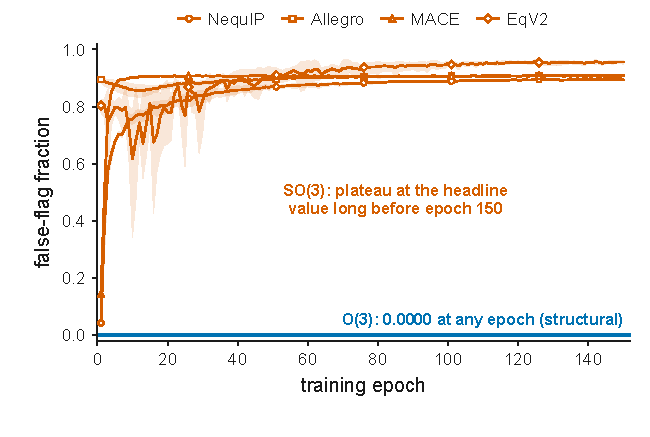
\includegraphics[width=0.62\textwidth]{figS1_epoch_curves}
\caption{False-flag fraction on the idealized centrosymmetric population as a function of training epoch, for the 12 re-instrumented SO(3) piezoelectric retrains (4 cores $\times$ 3 seeds; lines are seed means, bands the seed min--max, evaluated every epoch at the operating threshold). Every arm plateaus at its released headline value long before the epoch-150 budget; the O(3) arms are structurally zero at any epoch and any parameters, so they require no curve.}
\label{sfig:epochcurves}
\end{figure}

In the in-training control, the zero-labelled rows are fit better than the real-tensor rows (training MAE 0.014--0.045 versus 0.086--0.128 on targets whose mean component magnitude is 0.145), and training error on real rows is well below test error, so the models are neither ignoring the zeros nor underfitting.

\begin{table}[htbp]
\centering
\caption{Augmentation experiment: false-flag fraction (ff) and violation median on held-out centrosymmetric crystals from seen and unseen space groups, non-centrosymmetric test MAE, and the in-training control, before (baseline) and after (augmented) retraining the SO(3) arms; mean $\pm$ standard deviation over 3 seeds. The in-training column is the false-flag fraction on the 1,016 crystals carrying explicit zero labels in training (1,000 injected plus 16 real), the values quoted in the main text, re-derived from the augmentation run checkpoints. O(3) rows are the headline runs, not retrained, and are structurally zero.}
\label{stab:e1}
\fontsize{6bp}{7.5bp}\selectfont
\begin{tabular*}{\textwidth}{@{\extracolsep{\fill}}l rr rr rr@{}}
\toprule
 & \multicolumn{2}{c}{False-flag fraction} & \multicolumn{2}{c}{Violation median} & \\
\cmidrule(lr){2-3}\cmidrule(lr){4-5}
Core / arm & seen & unseen & seen & unseen & test MAE & ff trained zeros \\
\midrule
NequIP O(3) & $0.0000 \pm 0.0000$ & $0.0000 \pm 0.0000$ & $3.3\times10^{-7}$ & $2.9\times10^{-7}$ & $0.2083 \pm 0.0077$ & -- \\
NequIP SO(3) base & $0.9042 \pm 0.0021$ & $0.8811 \pm 0.0040$ & $0.826$ & $0.422$ & $0.2405 \pm 0.0080$ & -- \\
NequIP SO(3) aug. & $0.9042 \pm 0.0024$ & $0.8685 \pm 0.0039$ & $0.449$ & $0.254$ & $0.2278 \pm 0.0015$ & $0.895 \pm 0.0020$ \\
Allegro O(3) & $0.0000 \pm 0.0000$ & $0.0000 \pm 0.0000$ & $4.0\times10^{-7}$ & $3.4\times10^{-7}$ & $0.2140 \pm 0.0058$ & -- \\
Allegro SO(3) base & $0.9075 \pm 0.0000$ & $0.9128 \pm 0.0039$ & $1.182$ & $0.586$ & $0.2589 \pm 0.0176$ & -- \\
Allegro SO(3) aug. & $0.9067 \pm 0.0000$ & $0.8919 \pm 0.0045$ & $0.538$ & $0.274$ & $0.2303 \pm 0.0038$ & $0.899 \pm 0.0006$ \\
MACE O(3) & $0.0000 \pm 0.0000$ & $0.0000 \pm 0.0000$ & $3.0\times10^{-6}$ & $2.3\times10^{-6}$ & $0.2222 \pm 0.0066$ & -- \\
MACE SO(3) base & $0.9075 \pm 0.0000$ & $0.9080 \pm 0.0020$ & $1.156$ & $0.508$ & $0.2567 \pm 0.0084$ & -- \\
MACE SO(3) aug. & $0.9067 \pm 0.0008$ & $0.8924 \pm 0.0015$ & $0.534$ & $0.259$ & $0.2221 \pm 0.0107$ & $0.896 \pm 0.0025$ \\
EqV2 SO(3) base & $0.9508 \pm 0.0048$ & $0.9670 \pm 0.0066$ & $0.543$ & $0.295$ & $0.2157 \pm 0.0096$ & -- \\
EqV2 SO(3) aug. & $0.9302 \pm 0.0049$ & $0.9353 \pm 0.0106$ & $0.149$ & $0.102$ & $0.1774 \pm 0.0060$ & $0.922 \pm 0.0050$ \\
\bottomrule
\end{tabular*}
\end{table}

The final column of Supplementary Table~\ref{stab:e1} reports the in-training control: evaluated on the 1,016 crystals carrying explicit zero labels in training, every arm still flags roughly nine in ten, and none approaches the exact zero. (The four-decimal agreement between NequIP's in-training control and its evaluation-population fraction in Supplementary Table~\ref{stab:distribution} is coincidental: at full precision the values are $0.895341$ and $0.895333$, computed on different populations from different checkpoints.)

\subsection*{Zero-injection sweep ($N_{\mathrm{zero}}$ learning curve)}

Supplementary Table~\ref{stab:t3}a extends the augmentation experiment to a five-point sweep of the number of zero-labelled centrosymmetric crystals in training, on the NequIP SO(3) configuration. The sets are nested, each smaller one a prefix of the larger, with the $N{=}1{,}000$ point being the Supplementary Table~\ref{stab:e1} augmentation set exactly, drawn from the same six seen space groups under the same disjointness and idealization protocol with the target normalization frozen throughout; $N{=}16{,}000$ exhausts the qualifying Materials Project candidates in those groups. Over the sweep the held-out violation median falls 8.7-fold while the held-out false-flag fraction moves by only about four percentage points, and the in-training control stays at $0.88$--$0.90$ for every $N \geq 1{,}000$, its median falling only about twofold, not monotonically, and remaining six times the threshold at the largest feasible $N$: the loss-weight lesson, that approaching zero is not attaining it, reproduced along the data axis.

\begin{table}[htbp]
\centering
\caption{Augmentation sweeps (NequIP SO(3), mean $\pm$ s.d. over 3 seeds). a, Zero-injection sweep. ff, false-flag fraction at the operating threshold on the held-out 2,000 (global and split by whether the crystal's space group appears in the augmentation); median held-out, violation median on the held-out population; trained-zeros columns are the in-training control on the rows carrying explicit zero labels, $N$ injected plus the 16 real zero tensors already in the training set. Medians in C\,m$^{-2}$. $N{=}0$ is the headline run and $N{=}1{,}000$ the augmentation run of Supplementary Table~\ref{stab:e1}. b, Loss-weight sweep on the augmented training set. ff, false-flag fraction; median is the violation median on the 1,016 trained-on zero-labelled crystals in C\,m$^{-2}$. $W = 1$ is the augmentation run of Supplementary Table~\ref{stab:e1}.}
\label{stab:t3}

{\centering a, Zero-injection sweep\par}
\vspace{2pt}
\centering
\fontsize{7bp}{8.5bp}\selectfont
\begin{tabular*}{\textwidth}{@{\extracolsep{\fill}}rrrrrrr}
\toprule
$N_{\mathrm{zero}}$ & ff held-out & ff seen & ff unseen & median held-out & ff trained zeros & median trained zeros \\
\midrule
0 & $0.8953 \pm 0.0008$ & $0.9042$ & $0.8811$ & 0.666 & -- & -- \\
250 & $0.8937 \pm 0.0034$ & $0.9058$ & $0.8741$ & 0.522 & $0.7519 \pm 0.0038$ & $0.116$ \\
1{,}000 & $0.8905 \pm 0.0030$ & $0.9042$ & $0.8685$ & 0.373 & $0.8953 \pm 0.0020$ & $0.120$ \\
4{,}000 & $0.8818 \pm 0.0035$ & $0.9018$ & $0.8498$ & 0.178 & $0.8865 \pm 0.0014$ & $0.086$ \\
16{,}000 & $0.8582 \pm 0.0201$ & $0.8904$ & $0.8064$ & 0.077 & $0.8827 \pm 0.0109$ & $0.064$ \\
\bottomrule
\end{tabular*}

\vspace{8pt}
{\centering b, Loss-weight sweep\par}
\vspace{2pt}
\centering
\fontsize{7bp}{8.5bp}\selectfont
\begin{tabular*}{\textwidth}{@{\extracolsep{\fill}}rrrrrr}
\toprule
$W$ & ff trained zeros & median trained zeros & ff seen & ff unseen & test MAE \\
\midrule
1 & $0.8953 \pm 0.0020$ & 0.1200 & $0.9042 \pm 0.0024$ & $0.8685 \pm 0.0039$ & $0.2278 \pm 0.0015$ \\
10 & $0.8730 \pm 0.0026$ & 0.0463 & $0.9031 \pm 0.0012$ & $0.8420 \pm 0.0072$ & $0.2180 \pm 0.0027$ \\
100 & $0.6762 \pm 0.0154$ & 0.0140 & $0.8715 \pm 0.0031$ & $0.7604 \pm 0.0060$ & $0.2142 \pm 0.0055$ \\
\bottomrule
\end{tabular*}
\end{table}

\subsection*{Loss-weight sweep}

Supplementary Table~\ref{stab:t3}b tabulates the loss-weight sweep reported in the main text: the 1,016 exactly-zero rows up-weighted by $W$ in the loss. Even at $W = 100$ the model false-flags two-thirds of the crystals it was trained to call zero; the violation median on those crystals shrinks about ninefold yet remains four orders of magnitude above the O(3) floor, while the regression error slightly improves. Approaching zero is not attaining it; only the parity-labelled structure delivers exactness, at any weight.

% ===== Test-time inversion averaging =====

\subsection*{Test-time inversion averaging}\label{snote:inversion}

The proposed test-time repair antisymmetrizes the prediction over inversion, $T_{\mathrm{sym}}(x) = [T(x) - T(I\!\cdot\!x)]/2$. On an exactly centrosymmetric input, $I\!\cdot\!x$ is the same periodic crystal up to an atom permutation and a lattice translation, so any permutation- and translation-invariant model returns $T(I\!\cdot\!x) = T(x)$, verified to relative residual $10^{-6}$ for the three matched cores, and $T_{\mathrm{sym}}$ vanishes identically, for either parity arm, regardless of what the model has learned. The measurement corrected an expectation we held going in: we assumed the raw coordinate variant, being centrosymmetric only to tolerance, would retain signal under symmetrization; it does not, and the false-flag collapse occurs on both variants. Neither zero is evidence that symmetrization restores parity information; the construction succeeds for a reason that carries none.

Two costs remain even where the collapse occurs: inference is doubled, and the construction presupposes knowing the target's parity in advance: if the target were parity-even, the correct combination would be the symmetric one, and applying the antisymmetric projection would destroy the prediction. That knowledge is exactly what O(3) features encode per feature, everywhere, for every derived quantity at once.

EqV2 is the exception that proves the mechanism: its false-flag fraction falls only from about 0.95 to about 0.82, because it violates the permutation-invariance identity the fix relies on, its relative residual $|T(I\!\cdot\!x) - T(x)|/|T|$ being 0.10--0.15 rather than $10^{-6}$ (Supplementary Note~\ref{snote:eqv2}). The one deployed rotation-only model in this study is the one the proposed fix does not repair.

Quantitatively, on the idealized variant the symmetrized false-flag fraction is exactly $0.0000$ for all three matched cores in both parity arms (unsymmetrized SO(3) fractions in Supplementary Table~\ref{stab:distribution}), with symmetrized violation medians at the arithmetic floor ($3.0\times10^{-7}$, $6.5\times10^{-7}$ and $2.4\times10^{-6}$\,C\,m$^{-2}$ for NequIP, Allegro and MACE); the raw variant differs only in the fourth decimal. EqV2 is the exception, falling only from $0.9550$ to $0.8222$ with its median reaching just $2.8\times10^{-2}$\,C\,m$^{-2}$; its forward pass redraws a random per-edge frame on every call, and the $0.9550$ here against $0.9570$ in Supplementary Table~\ref{stab:distribution} is stochastic evaluation variance under a fresh seeded draw shared by $T(x)$ and $T(I\!\cdot\!x)$, not a disagreement between experiments. Per-core, per-seed values for both coordinate variants accompany the code release.

% ===== Symmetry breaking, rotation subgroups, and named materials =====

% ===== Note 6 =====
\suppnote{Symmetry breaking, rotation subgroups, and named materials}\label{snote:named}

\subsection*{Symmetry-breaking sweep}

Supplementary Fig.~\ref{sfig:rutile} shows the continuous polar-distortion sweep behind the main-text mechanism result; the distortion protocol and per-frame symmetry verification are given in main-text Methods. The figure caption records the arithmetic floors and spurious SO(3) floors for the rutile TiO$_2$ path and for the two further symmetry-verified 4/mmm paths, rutile-type SnO$_2$ and anatase TiO$_2$, on which the separation reproduces.

\begin{figure}[htbp]
\centering
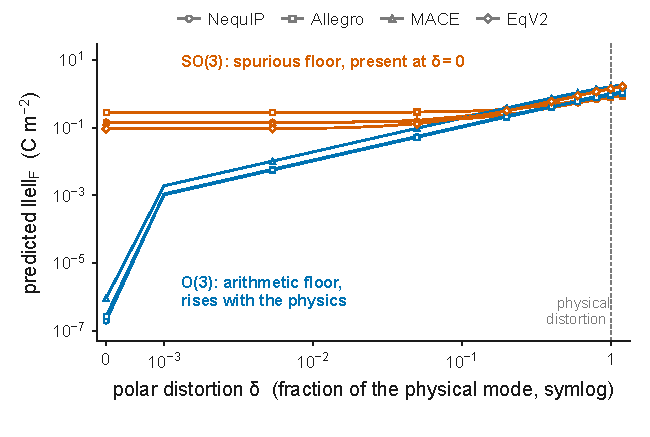
\includegraphics[width=0.62\textwidth]{figS2_rutile_sweep}
\caption{Predicted piezoelectric magnitude of rutile TiO$_2$ along a continuous polar distortion $\delta$ of the centrosymmetric parent, over 33 amplitudes, every frame symmetry-verified. The O(3) arms rise smoothly from the arithmetic floor ($1.9\times10^{-7}$ to $9.1\times10^{-7}$\,C\,m$^{-2}$ at $\delta=0$); the SO(3) arms sit on a spurious floor of 0.09--0.28\,C\,m$^{-2}$ that is present already at $\delta=0$ and dominates the physical signal throughout the small-distortion regime. The distortion axis is symmetric-log, matching the sweep's log-spaced amplitudes below $\delta = 0.05$, with a true zero for the centrosymmetric parent. The separation is not specific to rutile TiO$_2$. The sweep was repeated on two further symmetry-verified polar paths whose 4/mmm parents' rotation subgroup 422 likewise admits a rank-3 invariant: rutile-type SnO$_2$ (P4$_2$/mnm $\rightarrow$ P4$_2$nm) and anatase TiO$_2$ (I4$_1$/amd $\rightarrow$ I4$_1$md), every frame verified at symprec $10^{-8}$. On both, the O(3) arms again start at their arithmetic floor ($1.2\times10^{-7}$ to $1.2\times10^{-6}$\,C\,m$^{-2}$ at $\delta = 0$) while every SO(3) arm sits on a spurious floor of $0.04$--$1.25$\,C\,m$^{-2}$.}
\label{sfig:rutile}
\end{figure}

\subsection*{Rotation-subgroup analysis}

Supplementary Table~\ref{stab:e7} gives the per-family false-flag fractions behind main-text Fig.~4a. The group theory is verified numerically in the released test suite by Reynolds-operator rank tests: averaging a general rank-3 tensor over the proper-rotation subgroup 432 of point group m$\bar 3$m yields the zero map (projector rank 0), while averaging over subgroup 23 of point group m$\bar 3$ yields a one-dimensional invariant space (rank 1). Of the evaluation population, 1,834 of 2,000 crystals (the 18 of class m$\bar 3$ plus the 1,816 non-cubic ones, 91.7\%) lie outside what rotation alone can enforce, closely matching the observed SO(3) false-flag fractions. The SO(3) models' correct zeros are the ones rotations already guarantee; parity extends the guarantee to the strictly larger set that inversion demands.

\begin{table}[htbp]
\centering
\caption{False-flag fraction of the SO(3) arms by point-group family of the evaluated crystal (idealized variant, mean over 3 seeds; EqV2 over five evaluation draws per seed). Brackets give 95\% percentile-bootstrap confidence intervals over structures within each family (2,000 resamples, clustered by structure across seeds). The three matched O(3) arms are 0.0000 in every family and every seed.}
\label{stab:e7}
\scriptsize
\begin{tabular*}{\textwidth}{@{\extracolsep{\fill}}lrrr}
\toprule
Core (SO(3) arm) & m$\bar 3$m ($n{=}166$) & m$\bar 3$ ($n{=}18$) & non-cubic ($n{=}1{,}816$) \\
\midrule
NequIP & 0.0000 [0.0000,\,0.0000] & 0.9630 [0.9074, 1.0000] & 0.9765 [0.9704, 0.9824] \\
Allegro & 0.0000 [0.0000,\,0.0000] & 0.9815 [0.9444, 1.0000] & 0.9919 [0.9886, 0.9950] \\
MACE & 0.0000 [0.0000,\,0.0000] & 0.9444 [0.8519, 1.0000] & 0.9903 [0.9870, 0.9934] \\
EqV2 & 0.5341 [0.4679, 0.5984] & 0.9630 [0.8889, 1.0000] & 0.9956 [0.9936, 0.9976] \\
\bottomrule
\end{tabular*}
\end{table}

\subsection*{Named centrosymmetric materials}

Ten familiar centrosymmetric compounds were evaluated, the true piezoelectric tensor of every one being exactly zero. The O(3) prediction is at machine zero throughout, spanning $7.1\times10^{-10}$ to $2.5\times10^{-6}$\,C\,m$^{-2}$ across all ten compounds and three cores. The SO(3) predictions split exactly along the rotation-subgroup line of the preceding analysis: the class-m$\bar 3$m compounds (rocksalt, fluorite, caesium chloride, diamond-structure, cubic perovskite) are near zero for the exactly rotation-equivariant cores too, because their proper-rotation subgroup 432 already admits no rank-3 tensor, spanning $1.1\times10^{-9}$ to $1.5\times10^{-6}$\,C\,m$^{-2}$, while for the non-cubic compounds, corundum Al$_2$O$_3$ (sapphire) and rutile TiO$_2$, parity is the only remaining protection and every SO(3) model predicts $0.245$ to $1.128$\,C\,m$^{-2}$. EqV2's values on the m$\bar 3$m compounds span $5.8\times10^{-8}$ to $3.3\times10^{-2}$\,C\,m$^{-2}$, the nonzero end reflecting its approximate rotational equivariance (Supplementary Note~\ref{snote:eqv2}). Per-compound, per-core, per-seed values accompany the code release. Two caveats: the as-relaxed TiO$_2$ coordinates refine to space group 74 at the study tolerance, recovering the rutile group 136 only at looser tolerance (both centrosymmetric and non-cubic, leaving the interpretation unchanged; the analytically built rutile of the symmetry-breaking sweep is exactly group 136); and germanium is absent because its band gap in the source database falls below the insulator cut, so silicon stands in for the diamond-structure semiconductor.



\subsection*{Detection of responses in nominally centrosymmetric materials}

Sensitive resonance techniques do detect piezoelectric responses in nominally centrosymmetric materials~\cite{aktas2021nominally}, including NaCl and CaF$_2$, which appear in the named-materials table above. Those measurements report a real sample whose actual structure breaks inversion, whether or not an extrinsic cause is apparent, and their calibrated effective coefficients are orders of magnitude below conventional piezoelectrics, with the low-defect ionic crystals NaCl and CaF$_2$ at the very bottom of that range, below the detection limit of conventional measurement. The SO(3) violations reported here, by contrast, occur on exactly symmetric digital structures and reach the full magnitude of genuine piezoelectric tensors, so they are not the digital counterpart of that physical effect. The parity-labelled models capture the legitimate version of the phenomenon: the single raw-coordinate structure an O(3) arm flagged proved genuinely non-centrosymmetric below the selection tolerance, so the model responded to real symmetry breaking present in its input.

% ===== Prevalence audit =====

% ===== Note 7 =====
\suppnote{Prevalence audit of released architectures}\label{snote:audit}

Each of the eighteen released architectures in main-text Table~1 was classified by reading its released source at a pinned version or commit; the deciding evidence for every row is summarized in Supplementary Table~\ref{stab:audit}. Where source inspection could not settle the classification, the model was built and probed numerically. Two rows were converted from source-reading to measurement: ICTP~\cite{zaverkin2024ictp}, whose implicit Cartesian-harmonic parity was confirmed by a reflection test at random initialization (its rank-3 output is odd to machine precision, relative residual $0.0$, and its rank-2 output even), and GotenNet, which we suspected of discarding parity in its non-parity-typed attention blocks and which the measurement proved parity-aware: its degree-1 output obeys the polar-vector law under a random rotation (relative error $1.2\times10^{-15}$) and a random improper operation ($1.8\times10^{-15}$), while failing the pseudovector law ($1.9$). Parity is architectural, so probing at random initialization is sufficient.

The same reflection test was applied to the three vector-only rows, at random initialization in double precision (PaiNN~\cite{schutt2021painn} through schnetpack 2.2.0; TorchMD-Net (ET)~\cite{tholke2022torchmdnet} at the pinned commit, with its neighbour kernel replaced by an exhaustive pair list that does not touch the equivariant path; ViSNet~\cite{wang2024visnet} at the pinned torch-geometric release). In every case the node vector channel obeys the polar law $X(g\!\cdot\!x) = g\,X(x)$ under improper operations to machine precision (relative residuals $6\times10^{-16}$ to $4\times10^{-15}$) and violates the pseudovector alternative $\det(g)\,g\,X(x)$ by order unity: the channel is an untyped polar ($1o$) object, as its edge-vector construction implies. The classification is unchanged, since it records the absence of typed representations and of a rank-3 path rather than the absence of parity, but the load-bearing distinction is now measured rather than argued: these architectures carry parity implicitly while typing nothing, so a correctly assembled rank-3 readout would inherit the structural zero, whereas the SO(3)-only rows carry no parity information for any readout to recover.

The audit covers the current deployed generation directly: eSEN~\cite{fu2025esen}, the universal-potential family UMA~\cite{wood2025uma} that builds on it, and EqV3~\cite{equiformerv3}, whose title declares equivariance to SE(3), were classified by the same source-reading protocol at pinned versions and then measured by the same reflection test, at random initialization with the standard rank-3 readout attached (Theorem~1 holds at any parameter values, so no training is required). All three are SO(3)-only, and the measurement is unambiguous: each satisfies the rotation law to $2\times10^{-5}$--$1\times10^{-4}$ (single precision) and is bit-deterministic, yet violates the mirror law by order unity ($1.8$--$2.0$). On the 2,000-crystal population the random-initialized models already reproduce the rotation-ceiling signature: the m$\bar 3$m violation medians sit five to six orders of magnitude below the non-cubic medians (ratios $1.2\times10^{-6}$--$1.9\times10^{-5}$), with order-unity responses everywhere rotation does not forbid them. EqV3 is the informative case: it is exactly rotation-equivariant and deterministic, unlike EqV2, so its order-unity mirror violation removes the possibility that the headline behaviour of deployed spherical-channel models is an artefact of approximate equivariance.

\begingroup
\fontsize{7bp}{8.5bp}\selectfont
% Column widths are expressed against \textwidth rather than in cm so this table
% spans the text block exactly, matching every other table in the manuscript. The
% previous fixed cm widths rendered 348.8pt against a 372.0pt block. The reserve
% subtracted from the last column covers the natural-width `l` column (43.4pt as
% measured) plus the six \tabcolsep gaps between the four columns.
\begin{longtable}{@{}>{\raggedright\arraybackslash}p{0.168\textwidth} l >{\raggedright\arraybackslash}p{0.145\textwidth} >{\raggedright\arraybackslash}p{\dimexpr0.687\textwidth-61.4pt\relax}@{}}
\caption{Full prevalence audit. Classification of eighteen released architectures by the parity structure of their internal features, with the source version or commit inspected and the deciding evidence. Classes as in main-text Table~1. The unabridged evidence for every row, including the specific source file and line inspected, accompanies the code release.}
\label{stab:audit}\\
\toprule
Model & Class & Version / commit & Deciding evidence \\
\midrule
\endfirsthead
\toprule
Model & Class & Version / commit & Deciding evidence \\
\midrule
\endhead
\midrule
\multicolumn{4}{r@{}}{\itshape continued on next page}\\
\endfoot
\bottomrule
\endlastfoot
NequIP & parity-aware & 0.18.0 & Parity-labelled e3nn irreps; the preset \texttt{parity} boolean does not strip them. \\
Allegro & parity-aware & 0.8.3 & Parity-labelled e3nn irreps; \texttt{parity} flag documented to include odd features. \\
MACE & parity-aware & 0.3.16 & Natural-parity edge harmonics; \texttt{use\_so3=True} is the native all-even toggle. \\
MatTen~\cite{wen2024matten} & parity-aware & commit 0a04f1c & Default layer irreps carry both parities explicitly. \\
ICTP~\cite{zaverkin2024ictp} & parity-aware & commit f40592a & Implicit Cartesian-harmonic parity; rank-3 output measured odd to machine precision. \\
GotenNet~\cite{aykent2025gotennet} & parity-aware & commit 44c945b & Settled by measurement: polar law to $1.8\times10^{-15}$, pseudovector law failed ($1.9$). \\
\midrule
EquiformerV1 & SO(3)-only & commit 64cb786 & Default embeddings all-even; odd irreps only in auxiliary heads. \\
EquiformerV2 & SO(3)-only & vendored; upstream 8fe8cba & Degree/order-indexed embeddings, no parity; mirror-law violation confirmed (Supplementary Note~\ref{snote:eqv2}). \\
eSCN & SO(3)-only & vendored (Meta OCP lineage) & EqV2's embedding module; degree/order-typed, no parity label. \\
eSEN~\cite{fu2025esen} & SO(3)-only & fairchem-core 1.10.0 & Degree/order-typed coefficients; measured rotation $4\times10^{-5}$, mirror violated ($2.0$). \\
UMA~\cite{wood2025uma} & SO(3)-only & fairchem-core 2.21.0 & eSCN-lineage typing; measured rotation $1\times10^{-4}$, mirror violated ($1.8$). \\
EquiformerV3 \cite{equiformerv3} & SO(3)-only & commit a7300c5 & Degree-indexed, no parity; rotation-exact ($2\times10^{-5}$), deterministic, mirror violated ($2.0$). \\
\midrule
PaiNN~\cite{schutt2021painn} & vector-only & commit 2a2c913 & One unlabelled Cartesian vector channel; no typed irreps, no rank-3 path. \\
TorchMD-Net (ET)~\cite{tholke2022torchmdnet} & vector-only & commit 2a2c913 & Same vector channel; parity never represented. \\
ViSNet~\cite{wang2024visnet} & vector-only & torch-geometric 2.8.0 & Cartesian vector channel; no irreps anywhere. \\
\midrule
SchNet~\cite{schutt2017schnet} & invariant & torch-geometric 2.8.0 & Distance-only; invariant under all of O(3). \\
DimeNet++~\cite{gasteiger2020dimenetpp} & invariant & torch-geometric 2.8.0 & Distances and angles only; blind to mirror images. \\
FAENet~\cite{duval2023faenet} & invariant & commit 1f725cf & Not equivariant; frame averaging applied externally, improper frames a call-site choice. \\
\end{longtable}
\endgroup

% ===== Dedicated symmetry-enforcing predictors =====

% ===== Note 8 =====
\suppnote{Measurements on released models: dedicated predictors, frozen backbones, output-level audits, and cores not used}\label{snote:sota}

\subsection*{Dedicated symmetry-enforcing crystal-tensor predictors}

A parallel line of work enforces the correct tensor symmetry at the readout rather than in the features, through space-group-informed modules, canonicalization, or symmetry-adapted decompositions~\cite{yan2024gmtnet,goectp2024,lu2025eatgnn,piezotensornet2024,ceitnet2026}. Of the four current models of this kind, two release piezoelectric code and trained checkpoints: GMTNet~\cite{yan2024gmtnet} and CEITNet~\cite{ceitnet2026}, both built on an invariant backbone with the equivariant tensor synthesized only at the head. GoeCTP~\cite{goectp2024} and EATGNN~\cite{lu2025eatgnn} release only rank-2 dielectric implementations, whose parity-even target never exposes the parity-odd failure and whose piezoelectric variants are not available as published, so they cannot be evaluated on this test. We ran GMTNet and CEITNet on the same 2{,}000-crystal centrosymmetric population as the matched-pair experiment, through each model's own released pipeline at its released checkpoint, in two conditions: with the model's built-in space-group symmetry mask active (``mask on'') and disabled (``mask off''), and on both the idealized and the as-relaxed (raw) coordinates. Supplementary Table~\ref{stab:sota} reports the false-flag fraction (predicted magnitude above the $0.01$\,C\,m$^{-2}$ operating threshold; the true tensor is exactly zero for every crystal) in each condition.

\begin{table}[htbp]
\centering
\caption{Dedicated symmetry-enforcing predictors on the centrosymmetric population. False-flag fraction (fraction of the 2{,}000 crystals with predicted $\lVert e\rVert_F > 0.01$\,C\,m$^{-2}$; the true value is exactly zero for every crystal) for the two predictors that release piezoelectric checkpoints, with the built-in space-group mask on and off, on idealized and raw coordinates. The mask is the model's own symmetry-lookup repair; it is inert for the fully-forbidden point groups, where the head must already return zero unaided.}
\label{stab:sota}
\begin{tabular*}{\textwidth}{@{\extracolsep{\fill}}l l S[table-format=2.2] S[table-format=2.2]@{}}
\toprule
Model & Coordinates & {Mask off (\%)} & {Mask on (\%)} \\
\midrule
GMTNet  & idealized & 23.45 & 0.00 \\
GMTNet  & raw       & 21.70 & 1.05 \\
CEITNet & idealized & 11.95 & 9.15 \\
CEITNet & raw       & 11.00 & 9.35 \\
\bottomrule
\end{tabular*}
\end{table}

Two features of Supplementary Table~\ref{stab:sota} carry the argument: first, the two models rely on the mask very differently. GMTNet's mask repairs the idealized coordinates completely (from $23.45\%$ to $0.00\%$) but leaks to $1.05\%$ on the raw coordinates, where the space-group determination driving the symmetry lookup degrades: the repair is only as good as the symmetry oracle it consults, and real inputs erode that oracle. CEITNet's mask barely moves its rate ($11.95\%$ to $9.15\%$ idealized, $11.00\%$ to $9.35\%$ raw), because the mask is inert precisely for the fully-forbidden point groups, where the readout must already produce zero without help.

Second, the point-group family split inverts the pattern of the feature-based models. Splitting CEITNet's idealized mask-off predictions by family, it false-flags $68.7\%$ of the $166$ crystals of class m$\bar 3$m, and only $6.6\%$ of the $1{,}816$ non-cubic crystals where rotation alone does not forbid a response. The m$\bar 3$m class is the one every exactly rotation-equivariant model gets right by construction, because its proper-rotation subgroup $432$ alone forbids a rank-3 tensor (Corollary~\ref{scor:rot}). The predictor fails hardest exactly where rotation-equivariance would have succeeded, because the benchmark protocol these models are trained under removes symmetry-zero tensors from the training set, so the most strongly forbidden classes are the ones the model never sees. Readout-level repair therefore works exactly as far as its symmetry bookkeeping reaches; the structural guarantee either lives in the features, where it holds at any parameter values, or it is imposed from outside by an oracle that degrades on the inputs one actually encounters.

% ===== Frozen pretrained backbones =====

\subsection*{Inheritance through frozen pretrained backbones}\label{snote:frozen}

The matched-pair experiments toggle parity inside a network we build. Downstream practice increasingly does the opposite: it attaches a small property head to the frozen embeddings of a released universal potential, so the backbone's symmetry group is inherited rather than chosen. We measured that inheritance directly, under one protocol, on two released backbones that differ in exactly the property under test.

MACE-MP-0 small~\cite{batatia2023foundation} exposes parity-labelled features at the probe layer (\texttt{interactions.1.linear}, irreps $128{\times}0e+128{\times}1o+128{\times}2e+128{\times}3o$), so odd degrees are present and typed. eSEN-30M-OAM~\cite{fu2025esen,barrosoluque2024omat24} (checkpoint \texttt{esen\_30m\_oam.pt}, \texttt{facebook/OMAT24}) exposes $128{\times}0e+128{\times}1e+128{\times}2e+128{\times}3e$ at $l_{\max}=3$: the same degrees, every one declared even. Both feature spaces are 2,048-dimensional. In each case the backbone is frozen and only a linear equivariant readout to the piezoelectric irreps is trained (384 parameters on MACE-MP-0, 512 on eSEN), with Adam, learning rate $2\times10^{-3}$, 150 epochs, batch 16, no weight decay, three seeds, and the same splits and target normalization as the matched-pair runs. Feature extraction is deterministic to $0$ (MACE-MP-0) and $1.2\times10^{-6}$ (eSEN) across repeated passes.

The parity-labelled backbone transmits the guarantee intact: every one of the 2,000 centrosymmetric crystals returns an exact zero, in every seed, with a maximum violation of $0.0$ rather than an arithmetic floor, because a linear readout of parity-typed features cannot produce an odd-parity output from an inversion-invariant embedding. The parity-blind backbone transmits nothing: the same construction false-flags $0.900 \pm 0.004$ of the population, within the $0.90$--$0.96$ band of the matched SO(3) arms, at a violation median of $0.152$\,C\,m$^{-2}$ and a maximum of $2.6$\,C\,m$^{-2}$. Regression accuracy on the non-centrosymmetric test split is comparable, $0.158$ against $0.170$\,C\,m$^{-2}$ (a 7\% difference), so the two heads are equally competent regressors and differ only in whether the symmetry-forbidden zero survives (Supplementary Table~\ref{stab:frozen}).

A parity-even target would never have exposed the difference. Probed on the rank-2 dielectric tensor instead, both backbones would have passed, and the first parity-odd head attached later would have inherited the defect silently.

\begin{table}[htbp]
\centering
\caption{Piezoelectric head trained on frozen pretrained features, one protocol, two released backbones. Violations are on the 2,000-crystal centrosymmetric population where the true tensor is exactly zero; ff is the false-flag fraction at the operating threshold of $0.01$\,C\,m$^{-2}$. Mean $\pm$ s.d. over 3 seeds; medians and maxima in C\,m$^{-2}$.}
\label{stab:frozen}
\begin{tabular*}{\textwidth}{@{\extracolsep{\fill}}llrrrr@{}}
\toprule
Backbone & Feature parity & Head params & ff & median $\lVert e \rVert_F$ & max $\lVert e \rVert_F$ \\
\midrule
MACE-MP-0 small & parity-labelled & 384 & $0.0000$ & $0$ & $0$ \\
eSEN-30M-OAM & all-even & 512 & $0.8997 \pm 0.0042$ & $0.152 \pm 0.006$ & $2.605$ \\
\bottomrule
\end{tabular*}

\vspace{2pt}
{\fontsize{7bp}{8.5bp}\selectfont
Test MAE on the non-centrosymmetric split: MACE-MP-0 $0.1583 \pm 0.0000$, eSEN-30M-OAM $0.1697 \pm 0.0004$\,C\,m$^{-2}$. The MACE-MP-0 head is deterministic across seeds because the backbone is frozen and its readout has a unique least-squares solution on these features.\par}
\end{table}

% ===== Output-level audit and upstream reproduction =====

\subsection*{Output-level equivariance audit and EqV2 upstream reproduction}\label{snote:eqv2}

For every trained piezoelectric model, three output-level tests were run on the same structures: a mirror test comparing $T(Mx)$ with the parity-transformed prediction $D(M)\,T(x)$ for a random improper operation $M$, with $D$ built on the physical odd-parity irreducible representations; a rotation test with a random proper operation, which every arm must satisfy; and a determinism test of repeated forward passes on one input. The relative laws are measured on non-centrosymmetric structures, where the prediction is nonzero, since on a centrosymmetric input an O(3) model predicts machine zero and a relative error would divide floating-point noise. Supplementary Table~\ref{stab:eqv2audit} summarizes the results as ranges over seeds.

The O(3) arms satisfy the mirror law to floating-point precision; the SO(3) arms violate it by order unity, which is the parity defect measured directly at the output. Both arms of every matched core satisfy the rotation law and are bit-deterministic. EqV2 fails all three: its rotation-law error is 7--11\%, and it is the only nondeterministic model, because its forward pass draws a random per-edge reference frame on every call. For an exactly rotation-equivariant network the output would not depend on that arbitrary frame, so the determinism spread is itself a direct readout of rotational equivariance error; over five seeded draws of the full population evaluation, the median violation has a relative standard deviation of $6.5\times10^{-3}$ and the false-flag fraction a standard deviation of $5.0\times10^{-4}$, within which the single-draw headline value lies.

\begin{table}[htbp]
\centering
\caption{Output-level equivariance audit of every trained piezoelectric model: median relative errors over 25 non-centrosymmetric structures, shown as the range over 3 seeds. Mirror, violation of the improper-operation law; rotation, violation of the proper-rotation law; determinism, spread over five forward passes on one input.}
\label{stab:eqv2audit}
\centering
\fontsize{7bp}{8.5bp}\selectfont
\begin{tabular*}{\textwidth}{@{\extracolsep{\fill}}lllll}
\toprule
Core & Parity & Mirror & Rotation & Determinism \\
\midrule
NequIP & O(3) & $5.3$--$6.0\times10^{-7}$ & $0.9$--$1.1\times10^{-6}$ & $0.9$--$1.1\times10^{-6}$ \\
NequIP & SO(3) & $0.52$--$1.30$ & $0.9$--$1.0\times10^{-6}$ & $0.9$--$1.6\times10^{-6}$ \\
Allegro & O(3) & $8.2$--$9.2\times10^{-7}$ & $1.2\times10^{-6}$ & $2.1$--$7.3\times10^{-6}$ \\
Allegro & SO(3) & $1.11$--$1.17$ & $1.1$--$1.3\times10^{-6}$ & $4.6$--$11.0\times10^{-6}$ \\
MACE & O(3) & $3.0$--$3.8\times10^{-7}$ & $2.6$--$4.2\times10^{-6}$ & $0.8$--$1.4\times10^{-6}$ \\
MACE & SO(3) & $0.93$--$0.97$ & $3.0$--$3.9\times10^{-6}$ & $0.7$--$1.2\times10^{-6}$ \\
EqV2 & SO(3) & $0.71$--$0.98$ & $0.073$--$0.106$ & $0.111$--$0.144$ \\
\bottomrule
\end{tabular*}
\end{table}

To establish that the EqV2 findings are properties of the released code rather than of our packaging, all of them were reproduced against the pinned upstream repository (\texttt{atomicarchitects/equiformer\_v2}, commit \texttt{8fe8cba}, dated 2023-06-28, the only commit ever to touch the model files, which are frozen since). An abstract-syntax-tree comparison of all thirteen vendored model files against upstream found none differing substantively (six identical up to formatting, five up to import order, two carrying only documented dependency-removal edits), and the two load-bearing files, the per-edge reference-frame construction that is the source of the nondeterminism and the Wigner-matrix module whose detachment from atomic positions truncates the autograd Jacobian, are identical up to formatting and import order respectively.

The one executed method that does not originate in the upstream model files is the graph constructor, inherited upstream from an external base class; it was relocated into an auditable shim and proven inert by measurement: the shimmed upstream model reproduces the shipped vendored model bit-for-bit on a seeded forward pass (maximal absolute difference exactly zero), and replacing the shim by a hard stub returning the precomputed graph changes nothing. Reruns of the output-level audit on the shimmed upstream model with the trained checkpoints match the vendored values exactly to three decimals in every seed and every statistic (per-seed values accompany the code release), and an EqV2-specific finite-difference check confirms the incomplete autograd Jacobian on upstream source (relative disagreement 0.36--0.84, versus $9\times10^{-4}$ for NequIP under the identical check), which is the documented reason for its exclusion from the Jacobian analysis.

For context: the eSCN paper describes its SO(2) reduction as mathematically equivalent to the full convolution, that is, exact in theory; the frame-induced equivariance breaking is reported by users in the upstream issue tracker (issues 17 and 5 of the upstream repository). We report all of the above strictly as measured properties of the released code at the pinned commit and make no claim of incorrectness.

% ===== Models considered and excluded =====

\suppnote{Cores considered and not used, and a second non-e3nn O(3) control}\label{snote:excluded}\label{snote:hotpp}

Two further cores were considered and not used. EqV1's released dependency stack does not build for the GPU architecture used here, and as an e3nn-based model it exercises no mechanism the three matched cores do not already cover; EqV2 supersedes it as the transformer representative. A non-e3nn O(3)-equivariant core based on Clifford geometric algebra~\cite{polat2026cliffordstf}, intended to separate the headline effect from the e3nn implementation, was withdrawn for numerical conditioning rather than parity: it is O(3)-exact in exact arithmetic and cancels to order $10^{-15}$ on machine-perfect centrosymmetric input, but its algebra carries geometric grades only to degree 1, so a degree-3 output must pass through an ill-conditioned cubic tensor product, amplifying the order-$10^{-6}$ residual coordinate asymmetry of real crystals into a false-flag fraction of 0.42 that measures the readout's condition number, not the parity of the algebra.

That withdrawal leaves open whether any non-e3nn O(3) implementation can deliver the structural zero at the coordinate-noise scale of a real crystal, or whether the failure was general. We therefore tested a second, independently implemented non-e3nn core as a random-init structural control: HotPP~\cite{wang2024hotpp}, a Cartesian message-passing potential. It represents every rank-$k$ feature as a $k$-fold outer product of the unit bond vector, which is polar by construction with parity $(-1)^k$, and reaches its rank-3 output through a linear channel-mixing readout with no tensor product between input and output rank; the linear readout is the property whose absence disqualified the Clifford core. An exhaustive search of the package confirms it carries no e3nn dependency.

At random initialization in double precision, on the same nine idealized crystals of \snote{snote:sizeconsistency} fed through periodic neighbour lists, the summed rank-3 feature cancels to the double-precision noise floor on every crystal, at worst $4.0\times10^{-14}$ relative to a fixed per-atom reference scale, and the mirror law holds to machine precision (worst-case relative error $2.7\times10^{-15}$) on every crystal whose per-atom feature is not itself forced to zero by local site symmetry.

Because these idealized crystals are exactly centrosymmetric, with an inversion residual below $3\times10^{-15}$\,\AA{} rather than the $\sim10^{-6}$\,\AA{} of a relaxed structure, each was additionally displaced along a fixed random direction at $\varepsilon$ between $10^{-8}$ and $10^{-3}$\,\AA{} to emulate real coordinate noise, and the amplification factor that disqualified the Clifford core was measured: the relative output violation divided by the relative input displacement. HotPP's amplification is $2.2$--$21.5\times$, constant to better than $1.1\times10^{-4}$ relative deviation across five decades of $\varepsilon$, confirming a genuine linear response, against the $3{,}000$--$25{,}000\times$ of the Clifford core. That Clifford figure was measured on a trained model rather than at initialization, so the two are not a strictly matched comparison, but the three orders of magnitude separating them reflect the readout construction, which is fixed at every parameter value, rather than anything training supplies. One crystal, diamond-structure Si, is excluded from the statistic and reported separately: its violation scales as $\varepsilon^{2.00}$, a favourable cancellation arising from the local site symmetry of the diamond lattice rather than from conditioning.

This is a random-init structural control on nine idealized crystals, not a trained model evaluated on the 2,000-crystal population, and not a fourth arm of the matched-pair study. It establishes the narrower point that the structural zero survives in an implementation sharing no code with e3nn, and that the conditioning failure was a property of the Clifford readout rather than a general obstacle to non-e3nn O(3) implementations. Reproduced by \texttt{scripts/f4\_noneN3\_control.py}; full results in \texttt{results/f4\_noneN3\_control.json}.


\bibliography{references}

\end{document}
